\documentclass[12pt,a4paper]{report}

\usepackage{fontspec}
\usepackage[margin=2.5cm]{geometry}
\usepackage{setspace}
\usepackage{graphicx}
\usepackage{booktabs}
\usepackage{array}
\usepackage{tabularx}
\usepackage{longtable}
\usepackage{float}
\usepackage{caption}
\usepackage{subcaption}
\usepackage{enumitem}
\usepackage{amsmath,amssymb}
\usepackage[unicode,pdfpagelabels,plainpages=false]{hyperref}
\usepackage{xcolor}
\usepackage{fancyhdr}
\usepackage{pdfpages}
\usepackage{pdflscape}
\usepackage{rotating}
\usepackage{adjustbox}
\usepackage{polyglossia}
\setdefaultlanguage{english}
\setotherlanguage{arabic}
\setmainfont{Times New Roman}
\newfontfamily\arabicfont[Script=Arabic,Scale=1.08]{Arial}

\hypersetup{
    colorlinks=true,
    linkcolor=blue, 
    urlcolor=blue,
    citecolor=blue,
    pdftitle={MapIT - IT Infrastructure Documentation and Incident Knowledge Management},
    pdfauthor={MapIT Project Team}
}

\graphicspath{{figures/}{chapters/figures/}}

\setstretch{1.5}
\setlength{\parindent}{0pt}
\setlength{\parskip}{0.6em}

\pagestyle{fancy}
\fancyhf{}
\fancyhead[L]{MapIT}
\fancyhead[R]{\leftmark}
\fancyfoot[C]{\thepage}
\setlength{\headheight}{28pt}

\begin{document}

% -----------------------------------------------------------------------------
% Front matter
% -----------------------------------------------------------------------------
\hypersetup{pageanchor=false}
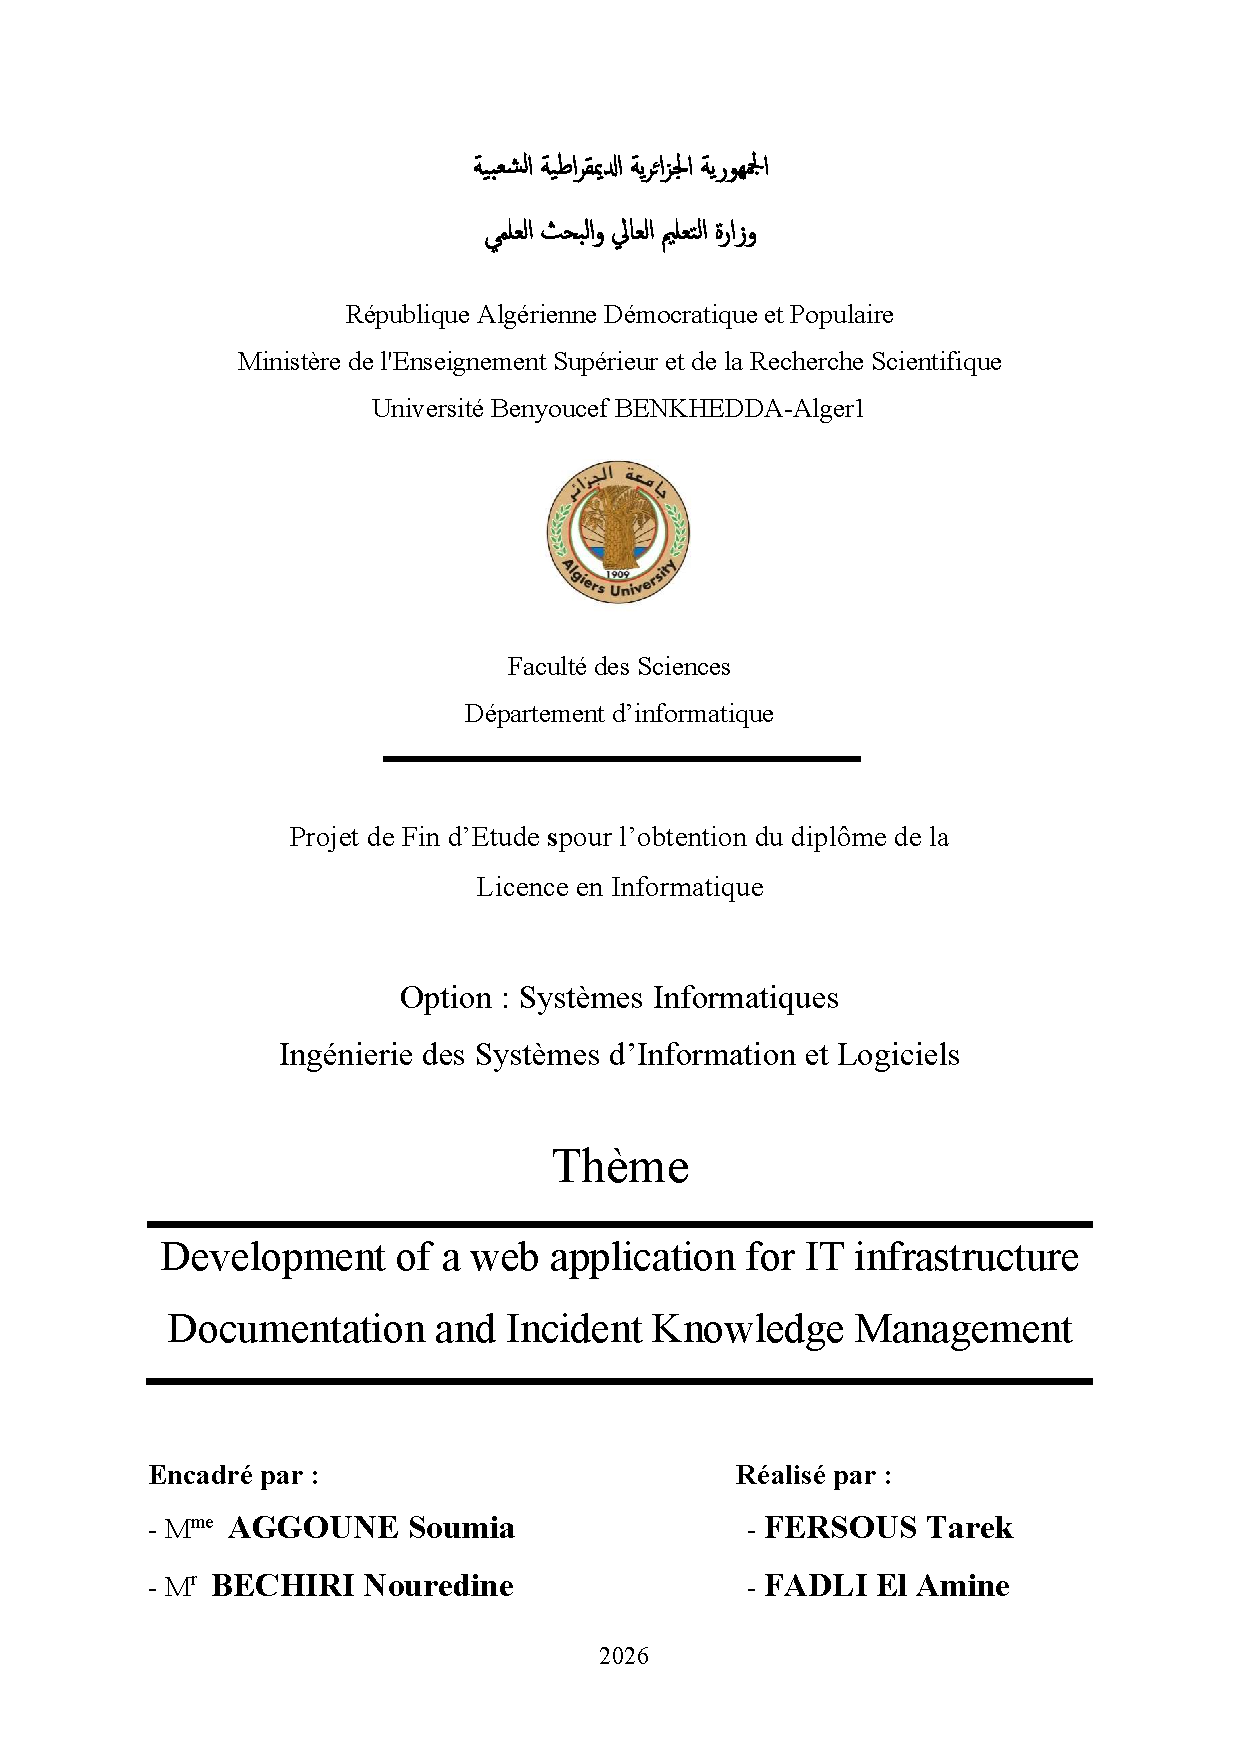
\includepdf[pages=1,fitpaper=true]{figures/page de garde.pdf}
\clearpage
\hypersetup{pageanchor=true}

\pagenumbering{roman}

\chapter*{Acknowledgements}
\addcontentsline{toc}{chapter}{Acknowledgements}
As we complete this work, we thank Allah for granting us the strength, patience, and clarity needed to carry it through.

We express our sincere gratitude to Ms. Soumia AGGOUNE for her guidance, availability, and constant encouragement throughout this project. Her support and precise advice helped us improve the work at every stage.

We also thank Mr. Nouredine BECHIRI, our external supervisor, for his valuable feedback, his thoughtful perspective, and the time he devoted to following our progress.

Our thanks extend to all the faculty members of the Computer Science Department for the knowledge and support they provided during our studies.

We are deeply grateful to our parents for their unconditional support, patience, and trust. Their encouragement made this journey possible.

Finally, we thank everyone who contributed directly or indirectly to the completion of this project.

\clearpage

\chapter*{Dedication}
\addcontentsline{toc}{chapter}{Dedication}

To my dearest mother, whose endless support, gentle presence, and unwavering belief have been my shelter through every storm—thank you for always standing by my side.

To my father, who raised me with strength and wisdom, showed me the path of integrity, and pushed me to become the person I am today—this achievement is as much yours as it is mine.

To my sweet younger sister, my anchor and my light, on whom I count in everything—thank you for being my constant source of joy and trust.

To my entire family, and especially my beloved grandmother, whose prayers never left my heart and whose motivation fueled my hardest days—I dedicate this work to you with all my love.

To the members of the Scientific University Club of Octobit and Open Source, for every line of code, every late-night discussion, and every moment of shared passion—you taught me more than I could ever put into words. The time spent with you was precious, and I carry it with me always.

To all my friends and university colleagues, and most especially to my PFE partner, who walked this final project journey with me step by step—thank you for your patience, collaboration, and camaraderie.

With deepest gratitude, this mémoire is yours as much as it is mine.


\vspace{1.5cm}
\hfill \textit{Tarek}

\clearpage

À mes parents \\
À mes frères \\
À mon binôme Tarek pour ses grands efforts

\vspace{0.5cm}
\hfill \textit{EL Amine}

\clearpage

\chapter*{Abstract}
\addcontentsline{toc}{chapter}{Abstract}
MapIT is a web-based platform created to bring together IT infrastructure documentation and incident knowledge management inside a single controlled workspace. It addresses a recurring operational weakness in support teams: notes are scattered, troubleshooting is repeated, and the link between an incident and the knowledge used to solve it is often lost. To reduce that fragmentation, the project combines a structured data model, role-based access control, and a clear user interface that supports incident registration, document maintenance, and reusable technical knowledge. The application is implemented as a full-stack system with a separated frontend, backend API, and relational database, making it the best choice for teams that need a lightweight but disciplined documentation environment.

\textbf{Keywords:} IT infrastructure, incident management, knowledge management, documentation platform, role-based access control.

\clearpage

\chapter*{\texorpdfstring{\hfill\textarabic{ملخص}}{ملخص}}
\addcontentsline{toc}{chapter}{\textarabic{ملخص}}
\begin{Arabic}
MapIT هي منصة قائمة على الويب تم إنشاؤها لجمع توثيق البنية التحتية لتكنولوجيا المعلومات وإدارة معارف الحوادث في مساحة عمل محكومة واحدة. وهي تعالج ضعفاً تشغيلياً متكرراً في فريق الدعم: الملاحظات متناثرة، واستكشاف الأخطاء مكرر، والربط بين الحادث والمعرفة المستخدمة لحله غالباً ما يكون مفقوداً. لتقليل هذا التجزئة، يجمع المشروع بين نموذج بيانات منظم، وتحكم في الوصول على أساس الأدوار، وواجهة مستخدم واضحة تدعم تسجيل الحوادث وصيانة المستندات والمعرفة التقنية القابلة لإعادة الاستخدام. يتم تنفيذ التطبيق كنظام متكامل مع واجهة أمامية منفصلة وواجهة برمجية خلفية وقاعدة بيانات علائقية، مما يجعله الخيار الأفضل للفرق التي تحتاج إلى بيئة توثيق خفيفة الوزن لكن منضبطة.

\textbf{الكلمات المفتاحية:} توثيق البنية التحتية لتكنولوجيا المعلومات، إدارة الحوادث، إدارة المعارف، منصة التوثيق، التحكم في الوصول على أساس الأدوار
\end{Arabic}
% Compact TOC layout without changing TOC content.
\chapter*{List of Abbreviations}
\addcontentsline{toc}{chapter}{List of Abbreviations}
\begin{itemize}[leftmargin=2cm]
    \item ITSM -- Information Technology Service Management
    \item CMDB -- Configuration Management Database
    \item UML -- Unified Modeling Language
    \item API -- Application Programming Interface
    \item CRUD -- Create, Read, Update, Delete
    \item DB -- Database
    \item LDAP -- Lightweight Directory Access Protocol
    \item ORM -- Object-Relational Mapping
    \item UI -- User Interface
    \item RBAC -- Role-Based Access Control
    \item JWT -- JSON Web Token
\end{itemize}

\clearpage

\begingroup
\setstretch{1.0}
\setlength{\parskip}{0pt}
\footnotesize
\tableofcontents
\endgroup
\clearpage
\addcontentsline{toc}{chapter}{List of Figures}
\begingroup
\setstretch{1.0}
\setlength{\parskip}{0pt}
\footnotesize
\listoffigures
\endgroup
\clearpage
\addcontentsline{toc}{chapter}{List of Tables}
\begingroup
\setstretch{1.0}
\setlength{\parskip}{0pt}
\footnotesize
\listoftables
\endgroup

\clearpage
\pagenumbering{arabic}

% -----------------------------------------------------------------------------
% Main body
% -----------------------------------------------------------------------------
\part{Theoretical Part}
\chapter{General Context and Introduction}

\section{Introduction}
MapIT is a full-stack application built to support the documentation of IT infrastructure, the management of incidents and assets, the mapping of relationships, and the reuse of technical knowledge. Rather than behaving like a generic document repository, the platform follows the daily logic of an IT support team: identify the asset, understand its dependencies, record the incident, preserve the resolution, and make that knowledge searchable for later reuse. This chapter situates the project in its real environment, states the problem it addresses, and explains why the topic matters both academically and professionally.
\section{Host Organization: SNTF}
\subsection{Short presentation}
SNTF stands for \emph{Société nationale des transports ferroviaires}, the Algerian state-owned company providing passenger and freight services using its extensive rail network. As per the company's official presentations, the SNTF was created in 1976, and reorganized in 1990 to become an EPIC entity.
\subsection{Visual identity}
Figure~\ref{fig:sntf-logo} presents the official SNTF logo used as a visual reference for the host organization.

\begin{figure}[H]
	\centering
	
\includegraphics[width=0.62\textwidth]{figures/sntf.png}
	\caption{Official logo of SNTF}
	\label{fig:sntf-logo}
\end{figure}

\subsection{DSI organigramme}
The DSI organigramme shows how the Information Systems Department is organized around several complementary missions: project management, network administration, systems development, web activities, database administration, security-oriented messaging and workstation support, and computer maintenance. This structure is useful for understanding where an internal documentation platform such as MapIT can support coordination between technical teams.

\begin{landscape}
\begin{figure}[p]
	\centering
	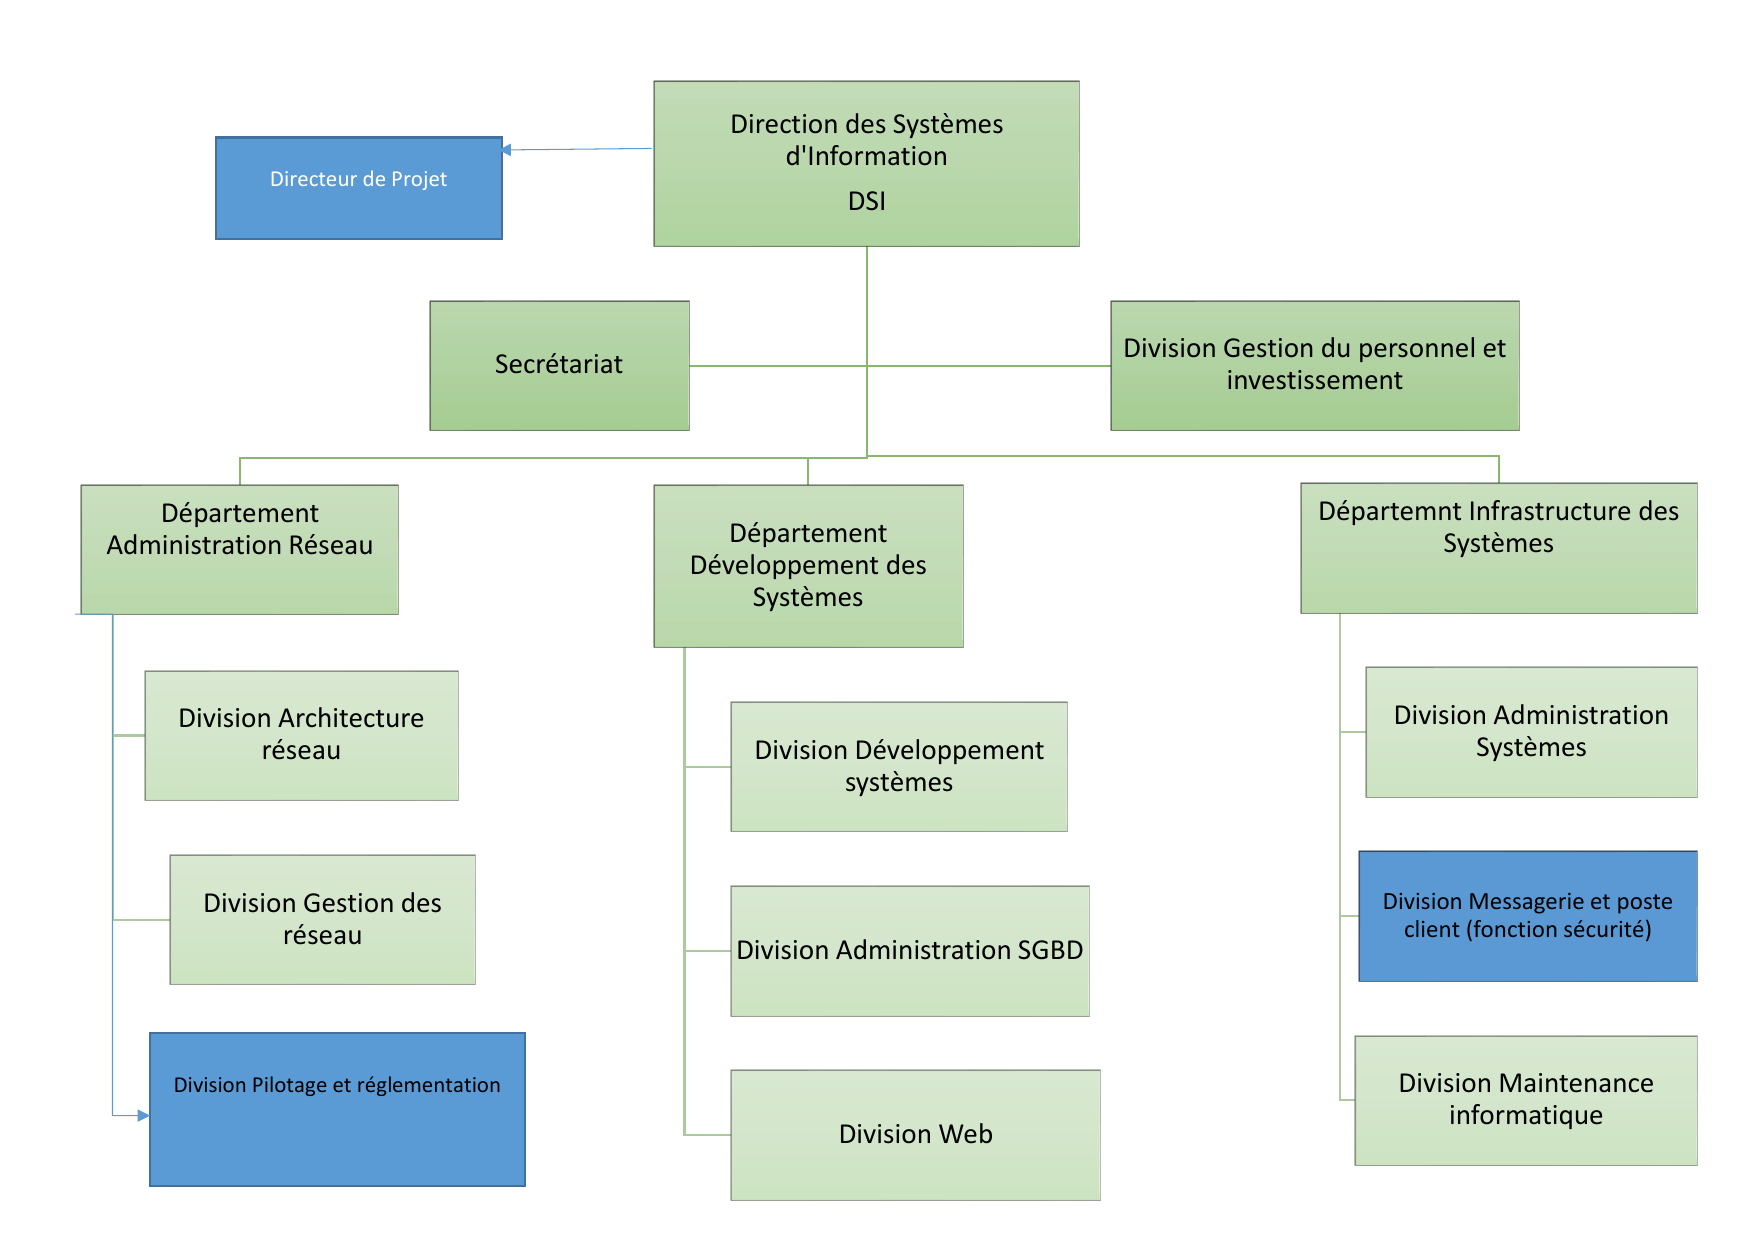
\includegraphics[height=0.86\textheight,keepaspectratio]{figures/dsi-organigramme.png}
	\caption{Organigramme of the SNTF DSI}
	\label{fig:sntf-dsi-organigramme}
\end{figure}
\end{landscape}

\subsection{Why SNTF is relevant to MapIT}
Given the nature of their business, a platform like MapIT would serve a natural purpose at SNTF. Railways depend on proper documentation, uninterrupted service, traceability, and coordination among the technical support teams. Operating a geographically dispersed transport network creates additional need to organize the knowledge systematically, and create visibility regarding assets, incidents, and inter-component relationships. Consequently, MapIT fits into the documentation requirements of a large enterprise.
\section{General Context}
In the world of today, IT infrastructures are deployed on servers, virtual machines, services, network devices, knowledge articles, and incident entries. In the codebase of MapIT, this diversity is evident in that there are specific routes for \texttt{/assets}, \texttt{/incidents}, \texttt{/problems}, \texttt{/relationships}, \texttt{/search}, \texttt{/reports}, and \texttt{/settings}, while the backend provides corresponding API modules for each domain. An IT platform in this environment requires more than merely displaying the data: it is meant to structure the technical memory for support specialists who are able to grasp dependencies, respond fast, and maintain the rationale behind their operations.
\section{Problem Statement}
\subsection{The operational gap}
The main problem solved by MapIT is the absence of a comprehensive, visualized environment for documenting knowledge about IT assets and incidents. In many real-life teams, asset data resides in one system, incident records live in another, and solutions are stored in yet a third source. The lack of integration makes it impossible for a support engineer to have the whole picture at hand: which asset was affected, which components depend on it, in which incident the same problem occurred before, and which document could be reused for the solution.

\subsection{Why the gap matters}
When the technical knowledge is fragmented into multiple documents, the same diagnostics has to be performed several times, the response is delayed, and organizational memories get lost. On top of that, it gets difficult to perform audits, assign responsibility, and track the progress of problem solving in time. In MapIT, these issues are handled through linking incidents with assets, problems, documents, and relationships, as well as through auditing permission related events.
\subsection{What is specific to MapIT}
MapIT is a specialized platform, not a generic content management system. It solves an issue with documentation in IT operations: lack of a single repository where knowledge would be available both in text and in graphs. The idea of linking an incident, problems, solutions, assets, and relations between them is precisely what makes MapIT unique. Thus, the operational gap that this project aims to fill is that of IT infrastructure knowledge management.
\section{Motivations and Project Relevance}
\subsection{Academic motivation}
From an academic point of view, the project is interesting since it combines major aspects of a specialization in Computer Systems: information systems analysis, relational data modeling, API design, authentication, access permissions, and front-end interface development. Following this logic, it can be seen that MapIT represents a good choice as a topic for an academic project.
\subsection{Professional motivation}
On a professional level, MapIT reflects the type of platform that technical support teams use for maintaining IT infrastructure. The platform includes a dashboard with summaries, asset inventory, incident life cycle management, knowledge/problem pages, graph visualization of relations, report generation, and access-controlled settings. This behavior is typical of knowledge platforms but not of brochure-like websites. Therefore, the project is relevant for a real-world IT environment and can be seen as a prototype for a practical solution to a common problem in the industry.
\section{Our Role as Computer Science Students Specializing in Computer Systems}
\subsection{Academic role}
As Computer Science students specializing in Computer Systems, our role was to turn a real operational need into a formal software architecture and then into a working implementation. This involved understanding the domain, defining the data model, specifying the access rules, and implementing the frontend and backend in a way that remains coherent and maintainable.

\subsection{Technical role}
The code shows that our technical role was broader than writing pages: we had to design the Prisma schema, implement JWT-based authentication with LDAP support in production and dev credentials in development, enforce permissions through middleware, and make the frontend consume the API through a Next.js proxy route. These tasks reflect a systems-oriented skill set because they connect infrastructure understanding with application engineering.

\section{Project Objectives and Scope}
\subsection{Functional objectives}
The immediate objectives of MapIT are to authenticate users, show an operational dashboard, manage assets, track incidents, document reusable problems and solutions, display infrastructure relationships, search across all knowledge types, and provide reporting and settings screens. The codebase confirms that each of these capabilities has a dedicated route and user interface.

\subsection{Scope of the first phase}
The current phase focuses on the essential operational workflow. It already includes login, dashboard summaries, incident list and detail views, asset inventory, knowledge/problem pages, relationship visualization, global search, reports, and settings. More advanced features such as richer analytics, automated workflows, or deeper notification logic can be introduced later without changing the core model.

\subsection{Planning and work organization}
The work was organized in successive phases: requirements analysis, study of existing solutions, theoretical framing, conception, modeling, implementation, and validation. This phased organization ensured that each deliverable was produced in the right order and that technical decisions remained aligned with the project objectives.

\section{Chapter Conclusion}
This chapter established that MapIT solves a concrete infrastructure knowledge problem: the absence of a centralized, visual, and role-aware place to manage assets, incidents, and reusable technical knowledge. The next chapter reviews the theoretical concepts that justify this architecture, especially information systems, knowledge management, incident tracking, and relationship mapping.

\chapter{Study of Existing Solutions}

\section{Introduction}
This chapter looks at tools and platforms that solve parts of the same problem space as MapIT. The point is not to collect names for the sake of completeness, but to understand how existing products treat documentation, incident traceability, collaboration, and knowledge reuse. That comparison gives the report a concrete baseline for the design choices made later.

\section{Methodology for Comparing Existing Solutions}
The comparison uses criteria that matter for an IT documentation and knowledge management platform. These criteria include structured organization, search quality, incident traceability, collaboration, access control, auditability, deployment flexibility, and licensing constraints. Using the same criteria for every product makes it possible to compare tools that were originally designed for very different audiences.

\section{Review of Existing Platforms}
Platforms such as ServiceNow, Jira Service Management, Confluence, GLPI, BookStack, Notion, SharePoint, and IT Glue show that the market already offers mature solutions for ticketing, documentation, and knowledge sharing. The common pattern is that each tool is strong in one direction and less complete in the others: service desk control, collaborative writing, enterprise content management, or flexible note keeping. For MapIT, the relevant question is whether a tool keeps infrastructure documentation and incident knowledge close together without turning the workflow into an oversized enterprise suite.

\section{Comparative Analysis}
The comparison table makes the differences visible at a glance. Enterprise tools are usually stronger in governance and workflow control, while lightweight tools are easier to adopt but weaker in traceability and structured access control. The conclusion is that MapIT is valuable precisely because it stays focused: it aims for clarity, controlled scope, and academic feasibility instead of reproducing the full breadth of a large commercial platform.

\begin{table}[H]
\centering
\small
\setlength{\tabcolsep}{3pt}
\renewcommand{\arraystretch}{1.12}
\begin{tabular}{|>{\raggedright\arraybackslash}p{2.35cm}|>{\raggedright\arraybackslash}p{3.85cm}|>{\raggedright\arraybackslash}p{3.85cm}|>{\raggedright\arraybackslash}p{3.85cm}|}
\hline
\textbf{Solution} & \textbf{Main strengths} & \textbf{Main limits} & \textbf{Relevance for MapIT} \\ \hline
\textbf{ServiceNow} & Mature ITSM workflows, governance, and automation. & Heavy, costly, and broader than the project scope. & Benchmark for rigor and access control. \\ \hline
\textbf{GLPI} & Open-source service desk with asset management. & Less oriented to relationship maps and reusable knowledge. & Useful for compact IT support comparison. \\ \hline
\textbf{Confluence} / BookStack & Strong structured documentation and collaboration. & Keeps documentation apart from incidents and dependencies. & Good reference for knowledge-base organization. \\ \hline
\textbf{Notion} & Flexible and easy for note-taking. & Weak structure, traceability, and IT-specific workflow control. & Shows limits of generic knowledge tools. \\ \hline
\textbf{MapIT} & Integrates assets, incidents, problems, relationships, search, and access control. & Deliberately narrower than enterprise suites. & Target solution of the study. \\ \hline
\end{tabular}
\caption{Feature comparison of existing solutions}
\label{tab:feature-comparison}
\end{table}

\section{Limitations of the Existing Approaches}
The reviewed approaches reveal several recurring limits. Some tools are expensive or too heavy for a compact academic deployment, while others are flexible but too generic to enforce a meaningful relationship between incidents and technical knowledge. In many cases, documentation is still separated from operational history, so the lesson learned from a previous incident is not naturally carried forward into the next one.

\section{Positioning of MapIT}
MapIT is positioned as a focused web application that covers the essential needs of infrastructure documentation and incident knowledge management without the overhead of a large enterprise suite. It is not meant to replace the market leaders. Its role is to show that a coherent solution can be tailored to the workflow of an IT team that needs controlled access, a clear relational model, and a direct connection between incidents and reusable knowledge.

\section{Chapter Conclusion}
This chapter shows that existing solutions address the problem only partially or at a broader scale than what the project requires. The comparison supports the decision to build MapIT as a compact, role-aware, and documentation-centric platform. The next chapter introduces the theoretical concepts that define the project domain.

\chapter{IT Infrastructure Documentation and Incident Knowledge Management}

\section{Introduction}
This chapter forms the theoretical bridge between the study of existing solutions and the practical implementation of MapIT. Its purpose is to define the concepts that make the project meaningful: information systems, knowledge management, incident tracking, and relationship mapping. These ideas are not abstract decorations; they correspond directly to the structure that appears in the codebase and in the user interface.

\section{Information Systems as a Knowledge Infrastructure}
\subsection{Definition of an information system}
An information system is an organized combination of people, processes, data, and technology that transforms raw data into usable information and supports operational decision-making \cite{laudon_mis,pressman}. In MapIT, this definition appears in the separation between the React/Next.js user interface, the Express backend API, the PostgreSQL database, and the permission middleware. The result is not just a website, but a small knowledge infrastructure for IT operations.

\subsection{Definition of IT documentation}
IT documentation can be defined as the structured and continuously maintained set of records that describes infrastructure components, operating procedures, dependencies, incidents, and decisions. Its role is to preserve operational memory so that technical teams can understand what exists, how it behaves, and what was done previously to maintain or restore it. In an IT service context, documentation is only useful when it is accurate, searchable, and tied to the real workflow of the organization \cite{itil4,km}.

Table~\ref{tab:it-doc-impact} summarizes the operational effect of documentation quality on daily IT work.

\begin{table}[H]
\centering
\small
\renewcommand{\arraystretch}{1.15}
\begin{tabular}{|p{0.30\textwidth}|p{0.30\textwidth}|p{0.30\textwidth}|}
\hline
\textbf{Feature} & \textbf{With Documentation} & \textbf{Without Documentation} \\ \hline
\textbf{Troubleshooting} & Fast, efficient & Slow, error-prone \\ \hline
\textbf{Onboarding} & Clear, structured & Confusing, inconsistent \\ \hline
\textbf{Compliance} & Easier to prove & Risk of violations \\ \hline
\textbf{Knowledge Sharing} & Smooth & Dependent on individuals \\ \hline
\textbf{System Reliability} & Higher & Lower \\ \hline
\end{tabular}
\caption{Impact of documentation on IT operations}
\label{tab:it-doc-impact}
\end{table}

\subsection{From data to operational knowledge}
MapIT stores data such as asset names, incident titles, problem descriptions, relationship types, and audit entries. That data becomes information when it is organized into pages, filters, status flows, or summary reports. It becomes operational knowledge when a technician can reuse it to answer a new incident, understand a dependency, or validate a corrective action. This progression is exactly why the application includes incidents, problems, documents, search, and feedback on knowledge suggestions.

Figure~\ref{fig:data-to-knowledge-chain} summarizes this progression in a simple visual chain.

\begin{figure}[H]
\centering
\fbox{\parbox{2.8cm}{\centering Raw data}}
\hspace{0.25cm}$\rightarrow$\hspace{0.25cm}
\fbox{\parbox{3.4cm}{\centering Structured information}}
\hspace{0.25cm}$\rightarrow$\hspace{0.25cm}
\fbox{\parbox{3.3cm}{\centering Operational knowledge}}
\hspace{0.25cm}$\rightarrow$\hspace{0.25cm}
\fbox{\parbox{2.8cm}{\centering Reuse and action}}
\caption{From data to reusable knowledge}
\label{fig:data-to-knowledge-chain}
\end{figure}

\subsection{Why the concept matters for MapIT}
The application is designed to preserve the technical memory of the infrastructure. A dashboard, a relationship graph, a search index, and a report summary all help the user see the system as a whole. In theoretical terms, MapIT is an information system that supports knowledge capture and knowledge retrieval in the same operational flow.

\section{Knowledge Management in IT Operations}
\subsection{Knowledge capture and reuse}
Knowledge management is the discipline of capturing experience, organizing it, validating it, and making it reusable \cite{davenport_prusak,nonaka_konno,km}. In MapIT, the reusable layer appears in problems with solutions, incidents with suggested knowledge, and documents that can be consulted later. The \texttt{IncidentKnowledgeFeedback} entity makes this process explicit by letting users state whether a suggested item was helpful.

\subsection{Knowledge quality and traceability}
Operational knowledge must be reliable, not merely available. That is why MapIT keeps audit logs, permission checks, and user-specific settings. The platform must know who changed a record, when it was changed, and under which permission level the action was executed. Without that traceability, the knowledge base would lose credibility in a real operational context.

\subsection{Why this is important for IT teams}
In an IT support environment, a good answer is not enough unless it can be found quickly and trusted. MapIT addresses this by indexing assets, problems, incidents, and documents through global search, by separating read access from management actions, and by exposing the operational state through a dashboard and reports. This is knowledge management as an operational practice, not just a repository.

\section{Incident Tracking and Relationship Mapping}
\subsection{Incident tracking}
Incident tracking is the formal recording of an incident from its opening to its closure, aligned with service management principles \cite{itil4,iso20000,atlassian_incident}. In the backend, MapIT uses a controlled incident lifecycle with the statuses \texttt{OPEN}, \texttt{IN\_PROGRESS}, \texttt{BLOCKED}, \texttt{RESOLVED}, and \texttt{CLOSED}. The detail page also supports priority, assignment, team ownership, and changes to status. This matters because it reflects the lifecycle discipline expected in modern service operations.

Figure~\ref{fig:incident-flow} illustrates the knowledge-reuse loop that follows an incident.

\begin{figure}[H]
\centering
	\fbox{\parbox{2.9cm}{\centering Incident record}}
	\hspace{0.2cm}$\rightarrow$\hspace{0.2cm}
	\fbox{\parbox{3.2cm}{\centering Root cause analysis}}
	\hspace{0.2cm}$\rightarrow$\hspace{0.2cm}
	\fbox{\parbox{3.0cm}{\centering Knowledge article}}
	\hspace{0.2cm}$\rightarrow$\hspace{0.2cm}
	\fbox{\parbox{2.8cm}{\centering Search and reuse}}
	\caption{Knowledge reuse cycle in IT operations}
\label{fig:incident-flow}
\end{figure}

\subsection{Relationship mapping}
Relationship mapping is the representation of dependency between infrastructure elements. In MapIT, relationships are stored as directed links between assets and visualized in a graph where the user can drag nodes, zoom, filter asset types, and inspect the connections. This feature is not decorative: it allows the user to reason about impact, identify upstream and downstream dependencies, and understand which asset relationships are affected by a failure.

\subsection{Why both concepts are essential}
Incident tracking gives the temporal view of a problem; relationship mapping gives the structural view of the infrastructure. Modern IT environments need both because a single incident can affect multiple assets, and a single asset can be implicated in multiple incidents over time. MapIT combines these two views so that the user can move from a symptom to a dependency to a reusable solution.

\section{Applying the Theory to MapIT}
\subsection{The MapIT domain model}
The Prisma schema shows how the theoretical concepts become concrete entities: \texttt{User}, \texttt{Incident}, \texttt{Document}, \texttt{Asset}, \texttt{Problem}, \texttt{Relationship}, \texttt{Role}, \texttt{Permission}, \texttt{AuditLog}, \texttt{UserSettings}, and \texttt{IncidentKnowledgeFeedback}. These objects reflect the real domain of the project and show that MapIT is centered on operational knowledge rather than on general content management.

Figure~\ref{fig:mapit-class-diagram} gives a schema view of these entities and their relationships.

\begin{figure}[H]
\centering
	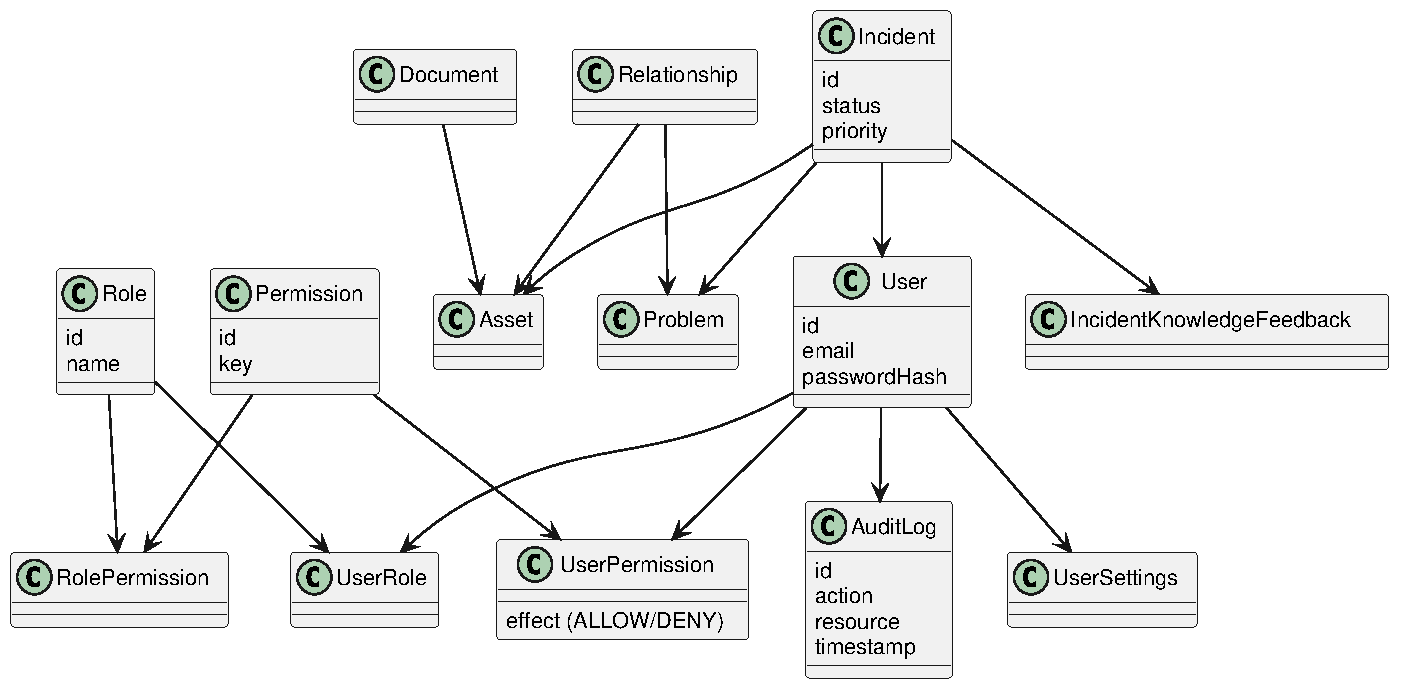
\includegraphics[width=0.95\textwidth]{figures/diagrams/simplified_class_diagram.pdf}
\caption{MapIT domain class diagram}
\label{fig:mapit-class-diagram}
\end{figure}

\subsection{How the theory appears in the interface}
The theory is visible in the frontend as well. The login page controls entry, the dashboard summarizes the environment, the incident detail page supports lifecycle actions, the asset pages show related problems and relationships, the search page unifies access to all knowledge, and the settings page exposes access control and audit logs. The access-control logic also follows common RBAC terminology used in enterprise systems \cite{microsoft_rbac}. This is the practical embodiment of the theoretical concepts defined in the chapter.

\subsection{Consistency of the theoretical path}
The theoretical path of this chapter moves from the definition of the domain to analysis, modeling, and realization. MapIT follows this logic through a practical IT infrastructure knowledge-management use case. The academic rigor is preserved by defining the concepts, justifying the approach, and showing how the implementation proves the model.

\section{Chapter Conclusion}
MapIT is grounded in established notions of information systems and knowledge management, but it applies them to a very specific IT operations problem: keeping infrastructure knowledge centralized, visual, and actionable. Incident tracking and relationship mapping are therefore core academic concepts for the project, not side features. The next chapter will show how these concepts were translated into the concrete software architecture and user-facing pages.


\part{Practical Part}
\chapter{Conception}

\section{Introduction}
This chapter converts the theoretical understanding of the domain into a concrete design for MapIT. The goal is to define what the system must do, how it should be organized, and which constraints guide the technical choices. The conception phase therefore bridges the gap between the problem statement and the formal modeling of the solution.

\section{Requirement Elicitation}
The expected needs of the platform were identified by examining the everyday tasks performed in documentation and incident-oriented IT workflows. This includes the need to consult knowledge quickly, register incidents with enough detail to be useful later, and keep the interface simple enough for non-specialists to use. The requirements were then separated into functional needs, which describe what the system must do, and non-functional needs, which describe how well it must do it.

\section{Functional Requirements}
The main functional requirements of MapIT are straightforward: users must authenticate securely, consult a dashboard, register incidents, create and update documentation entries, search content, and perform actions according to their role. Administrators must be able to manage sensitive operations, while standard users should still have access to the knowledge base and incident records required for their work. This definition keeps the first release focused on core operational value rather than peripheral features.

\section{Non-Functional Requirements}
Several non-functional qualities are important for this type of system. Security is necessary because the platform stores operational information and controls access to it; usability matters because the knowledge base must be easy to navigate under time pressure; maintainability is important because the application should remain understandable as it evolves; and traceability is needed so that users can trust the history of the data. Performance and reliability also matter, even in an academic prototype, because slow search or unstable access would immediately reduce adoption.

\section{High-Level Architecture}
MapIT follows a simple three-tier architecture composed of a frontend, a backend API, and a relational database. The frontend is responsible for the user experience, the backend handles business logic and authorization, and the database stores the structured records that support incidents, documents, and users. This separation improves maintainability and makes the system easier to evolve because each layer has a clear responsibility.

Figure~\ref{fig:architecture-mapit} presents the concrete architecture used in the project, including the web client, API server, and persistence layer.

\begin{figure}[H]

	\centering
	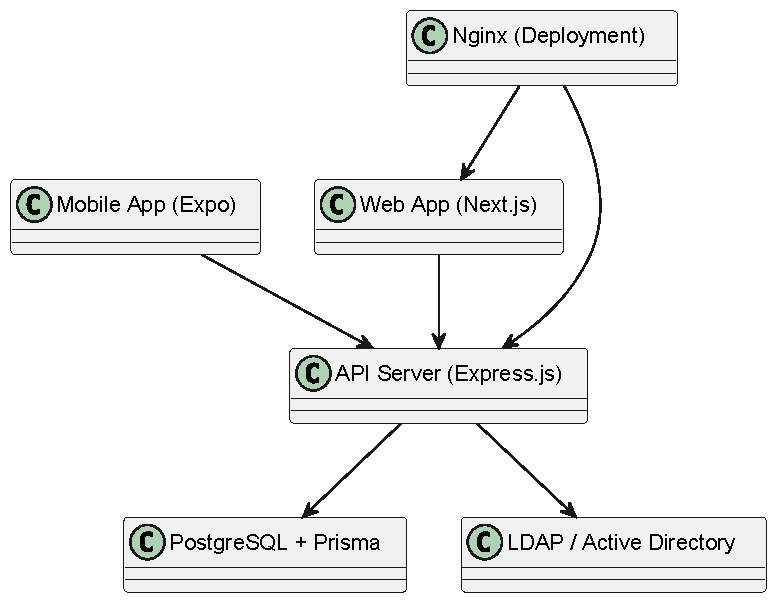
\includegraphics[width=0.95\textwidth]{figures/diagrams/architecture_diagram.pdf}
	\caption{High-level architecture of MapIT}
	\label{fig:architecture-mapit}
\end{figure}


\section{Module Decomposition and User Journeys}
The system is divided into modules that reflect the main business activities of the platform: authentication, dashboard visualization, incident management, document management, and administration. A typical user journey begins at login, continues with a dashboard overview, and then leads to either the creation of a new record or the consultation of an existing one. This modular design keeps the application understandable and allows each user role to follow a path that matches its responsibilities.

\section{Design Decisions and Constraints}
The design choices are driven by a need for data consistency, controlled access, and easy navigation. A centralized data model avoids duplication between incidents and documents, while role-based rules prevent unauthorized modification of critical records. At the same time, the interface must remain clean and direct so that the system can be used as a practical knowledge tool rather than as a purely theoretical database.

\section{Chapter Conclusion}
The conception phase establishes a clear functional direction for the application and frames the main constraints that the implementation must respect. It shows that MapIT is intentionally focused on the workflows that matter most for incident-oriented documentation. The next chapter formalizes this design through UML and data modeling artifacts.

\chapter{Modeling}

\section{Introduction}
This chapter formalizes MapIT through analysis and modeling artifacts. The diagrams and schemas presented here translate the conception choices into a precise structural view of the system. They are important because they make the behavior of the application easier to verify before implementation begins.

\section{Actors and Use Cases}
The use case model identifies the principal actors of the system, such as a standard user and an administrator, and shows how each role interacts with the application. The use case diagram provides a global view of the services offered by MapIT, including authentication, incident management, document management, and administrative operations. This representation helps the reader understand the scope of the system before entering into detailed scenarios.

Figure~\ref{fig:use-case-mapit} summarizes the interactions between users and the core services of the platform.

\begin{figure}[H]
	\centering
	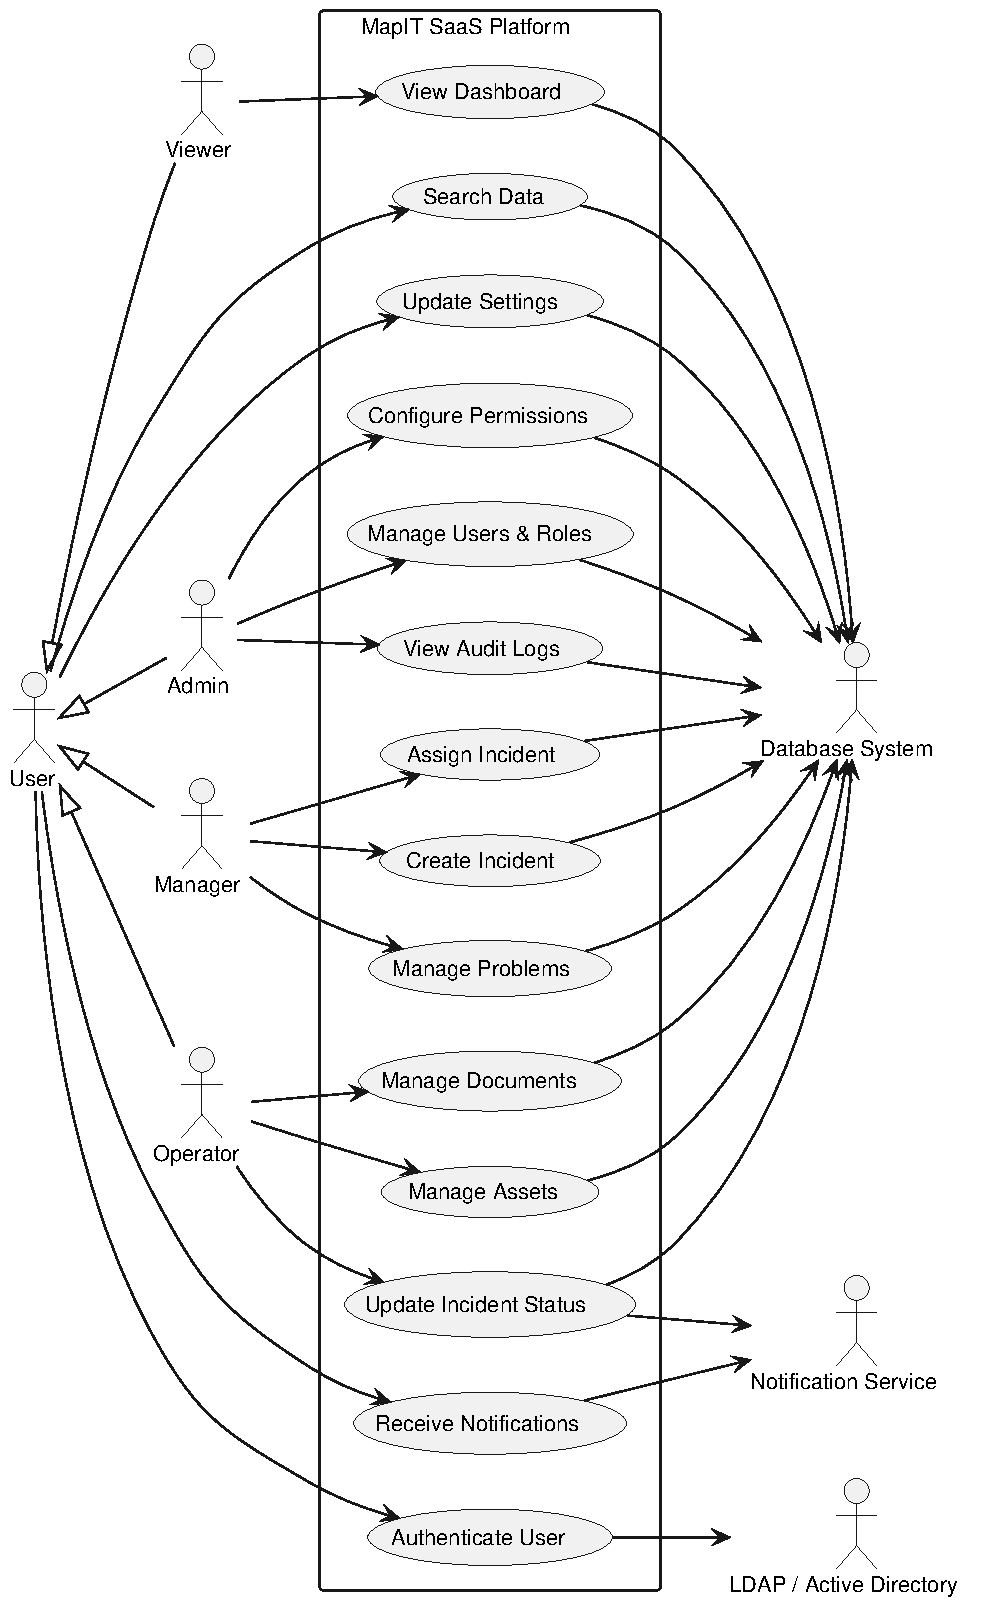
\includegraphics[width=0.92\textwidth]{figures/diagrams/updated_use_case_diagram.pdf}
	\caption{Use case diagram of MapIT}
	\label{fig:use-case-mapit}
\end{figure}

\section{Use Case Specifications}
Each major use case is described textually in terms of goal, actor, preconditions, main steps, alternate paths, and postconditions. This level of detail is important because it shows how the system behaves when a user logs in, creates a record, edits content, or performs a restricted action. The textual specification also serves as a useful reference during development and testing.

\section{Sequence Diagrams}
Sequence diagrams are used to describe the dynamic behavior of the system for representative scenarios such as authentication, incident creation, and document consultation. They show the message flow between the user interface, the API layer, the business logic, and the database, making it easier to verify that the architecture supports the intended user journeys. In an academic report, these diagrams also help demonstrate that the implementation follows a coherent interaction pattern.

The authentication interaction flow is shown in Figure~\ref{fig:seq-auth}.

\begin{figure}[H]
	\centering
	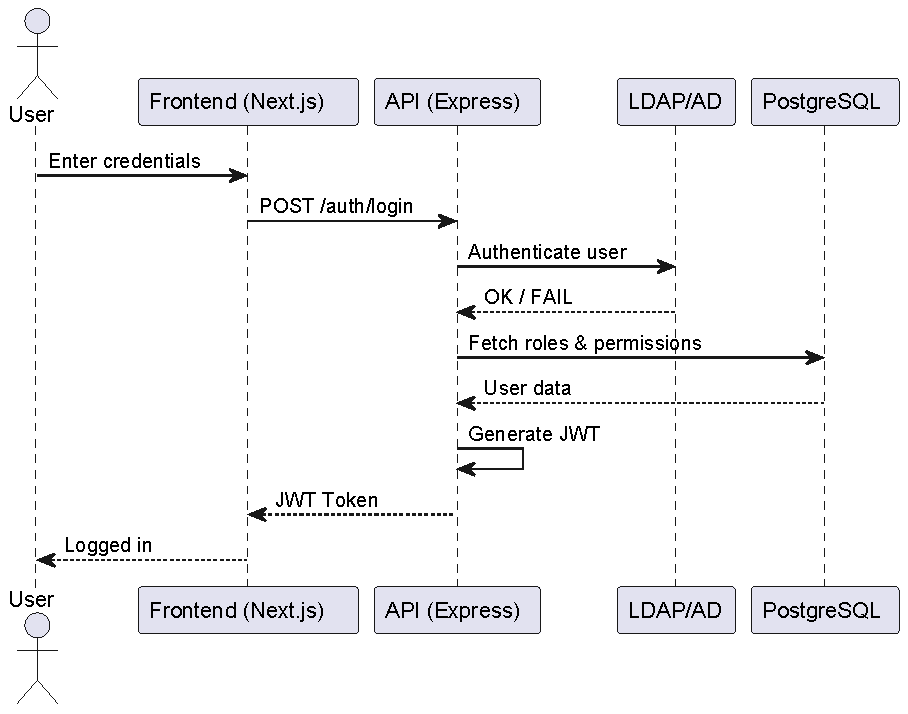
\includegraphics[width=0.95\textwidth]{figures/diagrams/sequence_diagram_authentication.pdf}
	\caption{Sequence diagram: authentication flow}
	\label{fig:seq-auth}
\end{figure}

The advanced authentication scenario, including session and permission checks, is shown in Figure~\ref{fig:seq-auth-advanced}.

\begin{landscape}
\begin{figure}[p]
	\centering
	\vspace*{\fill}
	\begin{adjustbox}{width=\linewidth, totalheight=0.8\textheight, keepaspectratio}
		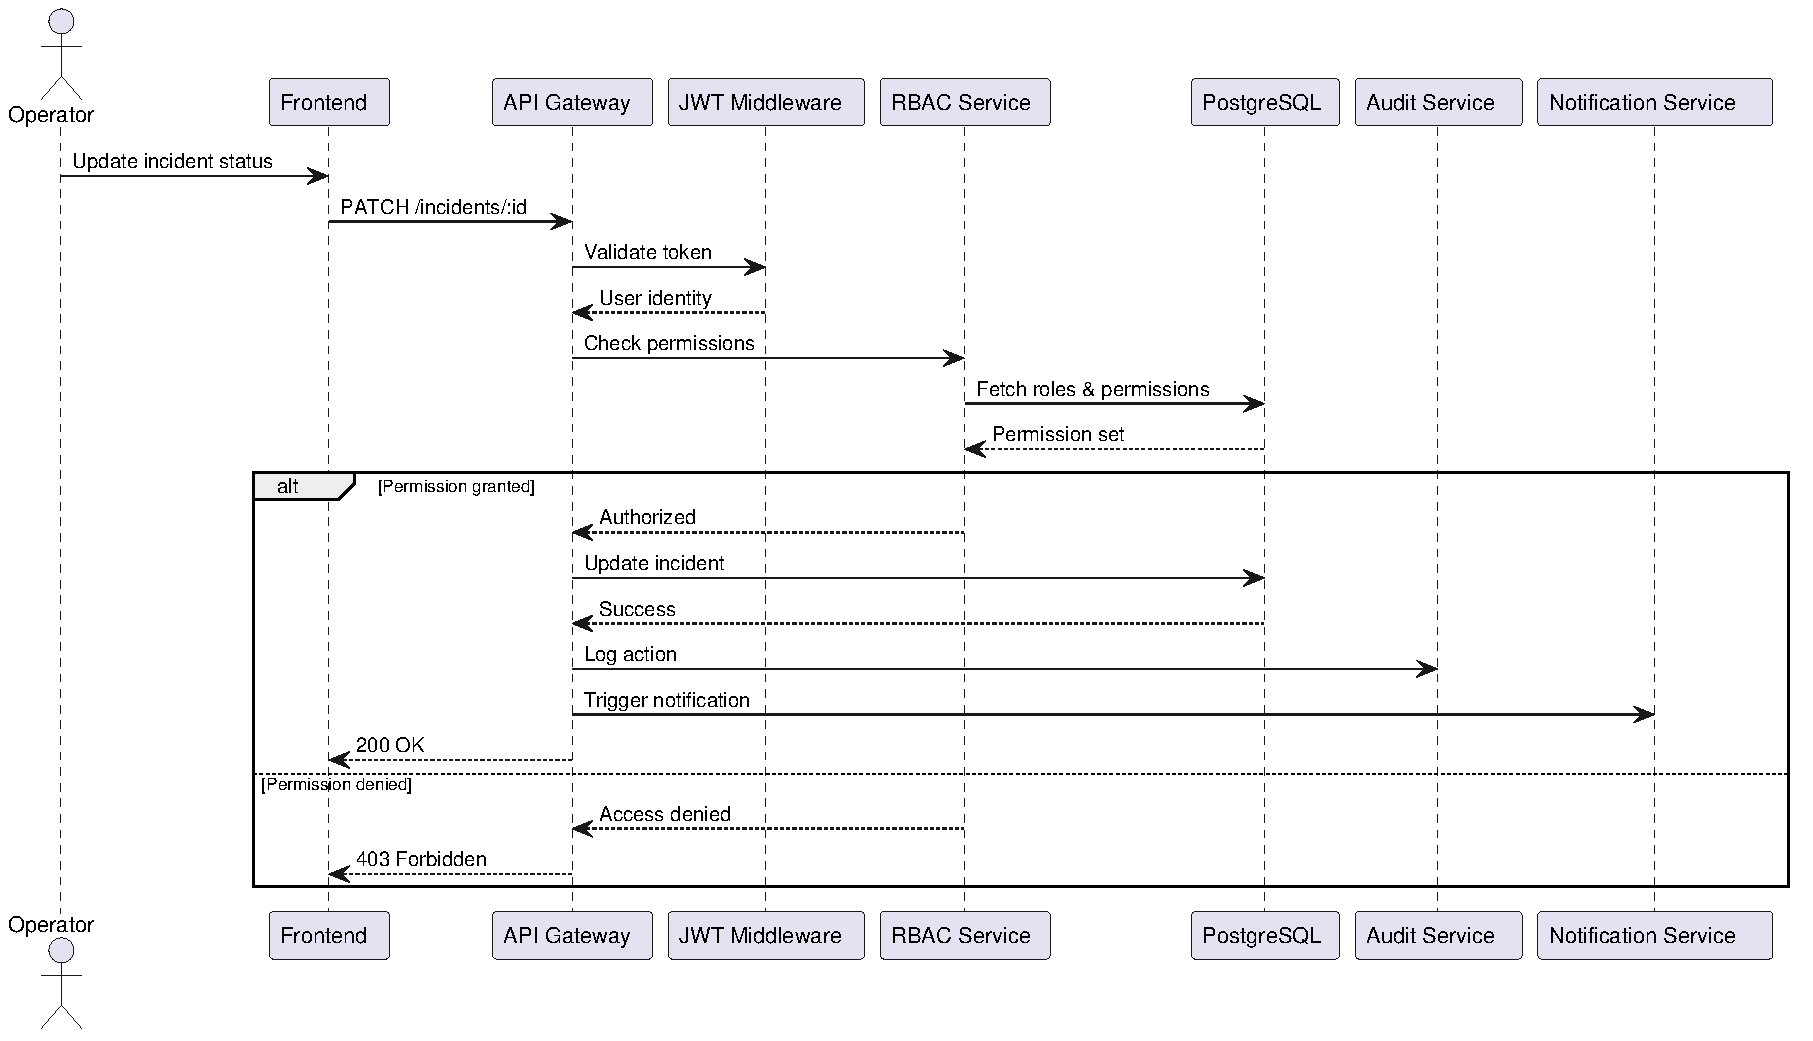
\includegraphics{figures/diagrams/advanced_auth_sequence_diagram.pdf}
	\end{adjustbox}
	\vspace*{\fill}
	\caption{Advanced authentication sequence diagram}
	\label{fig:seq-auth-advanced}
\end{figure}
\end{landscape}

The lifecycle of incident processing is detailed in Figure~\ref{fig:seq-incident}.

\begin{figure}[H]
	\centering
	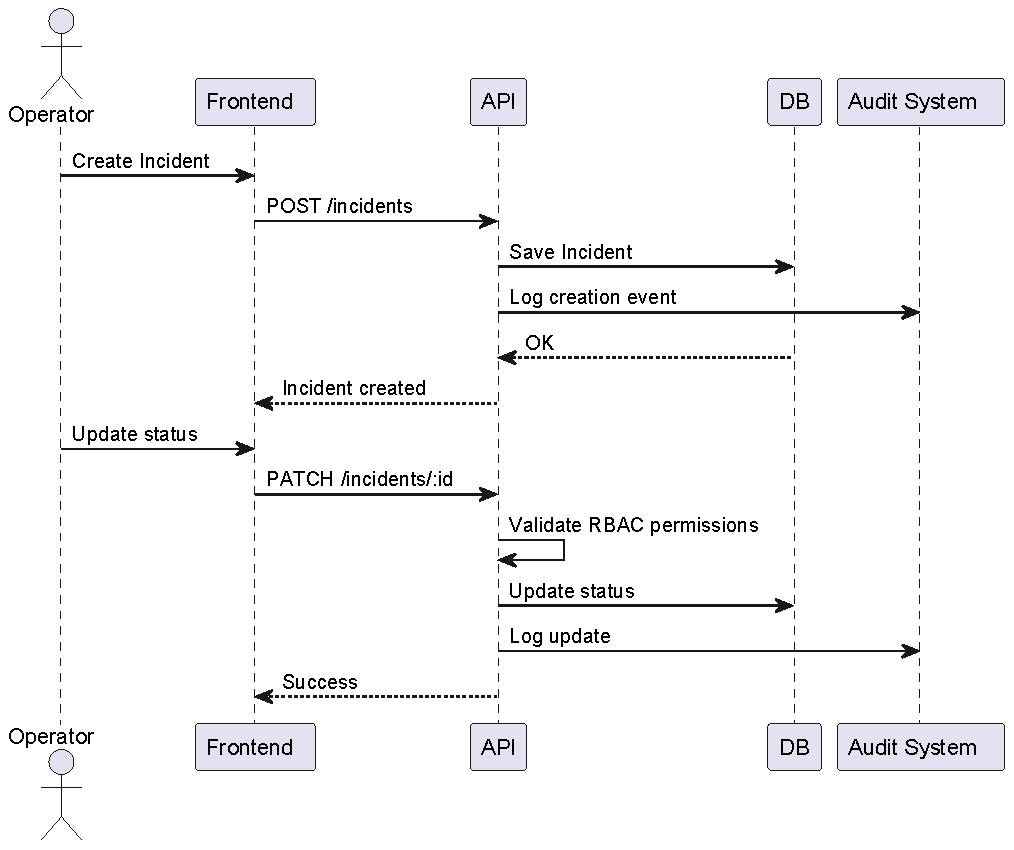
\includegraphics[width=0.95\textwidth]{figures/diagrams/sequence_diagram_incident_flow.pdf}
	\caption{Sequence diagram: incident management flow}
	\label{fig:seq-incident}
\end{figure}

The global search interaction, which aggregates multiple data domains, is presented in Figure~\ref{fig:seq-search}.

\begin{figure}[H]
	\centering
	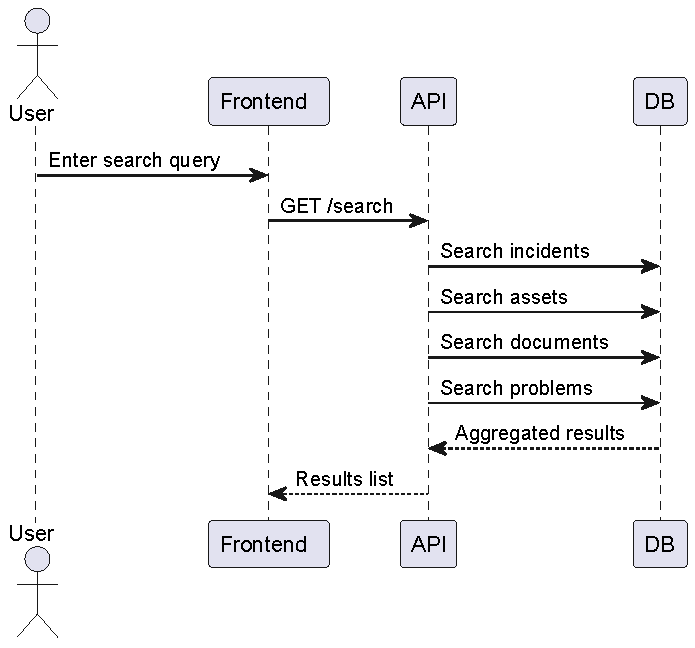
\includegraphics[width=0.95\textwidth]{figures/diagrams/sequence_diagram_global_search.pdf}
	\caption{Sequence diagram: global search flow}
	\label{fig:seq-search}
\end{figure}

\section{Class Diagram and Domain Model}
The class diagram captures the static domain structure of MapIT and presents the main entities of the application. Typical classes include User, Role, Incident, Document, Category, Comment, and AuditLog, together with the relationships that connect them. The diagram makes it clear which objects own data, which objects reference others, and how the domain supports both documentation and traceability.

Figure~\ref{fig:class-mapit} illustrates the domain model used to implement these entities and their associations.

\begin{landscape}
\begin{figure}[p]
    \centering
	\vspace*{\fill}
    \begin{adjustbox}{width=\linewidth, totalheight=0.8\textheight, keepaspectratio}
		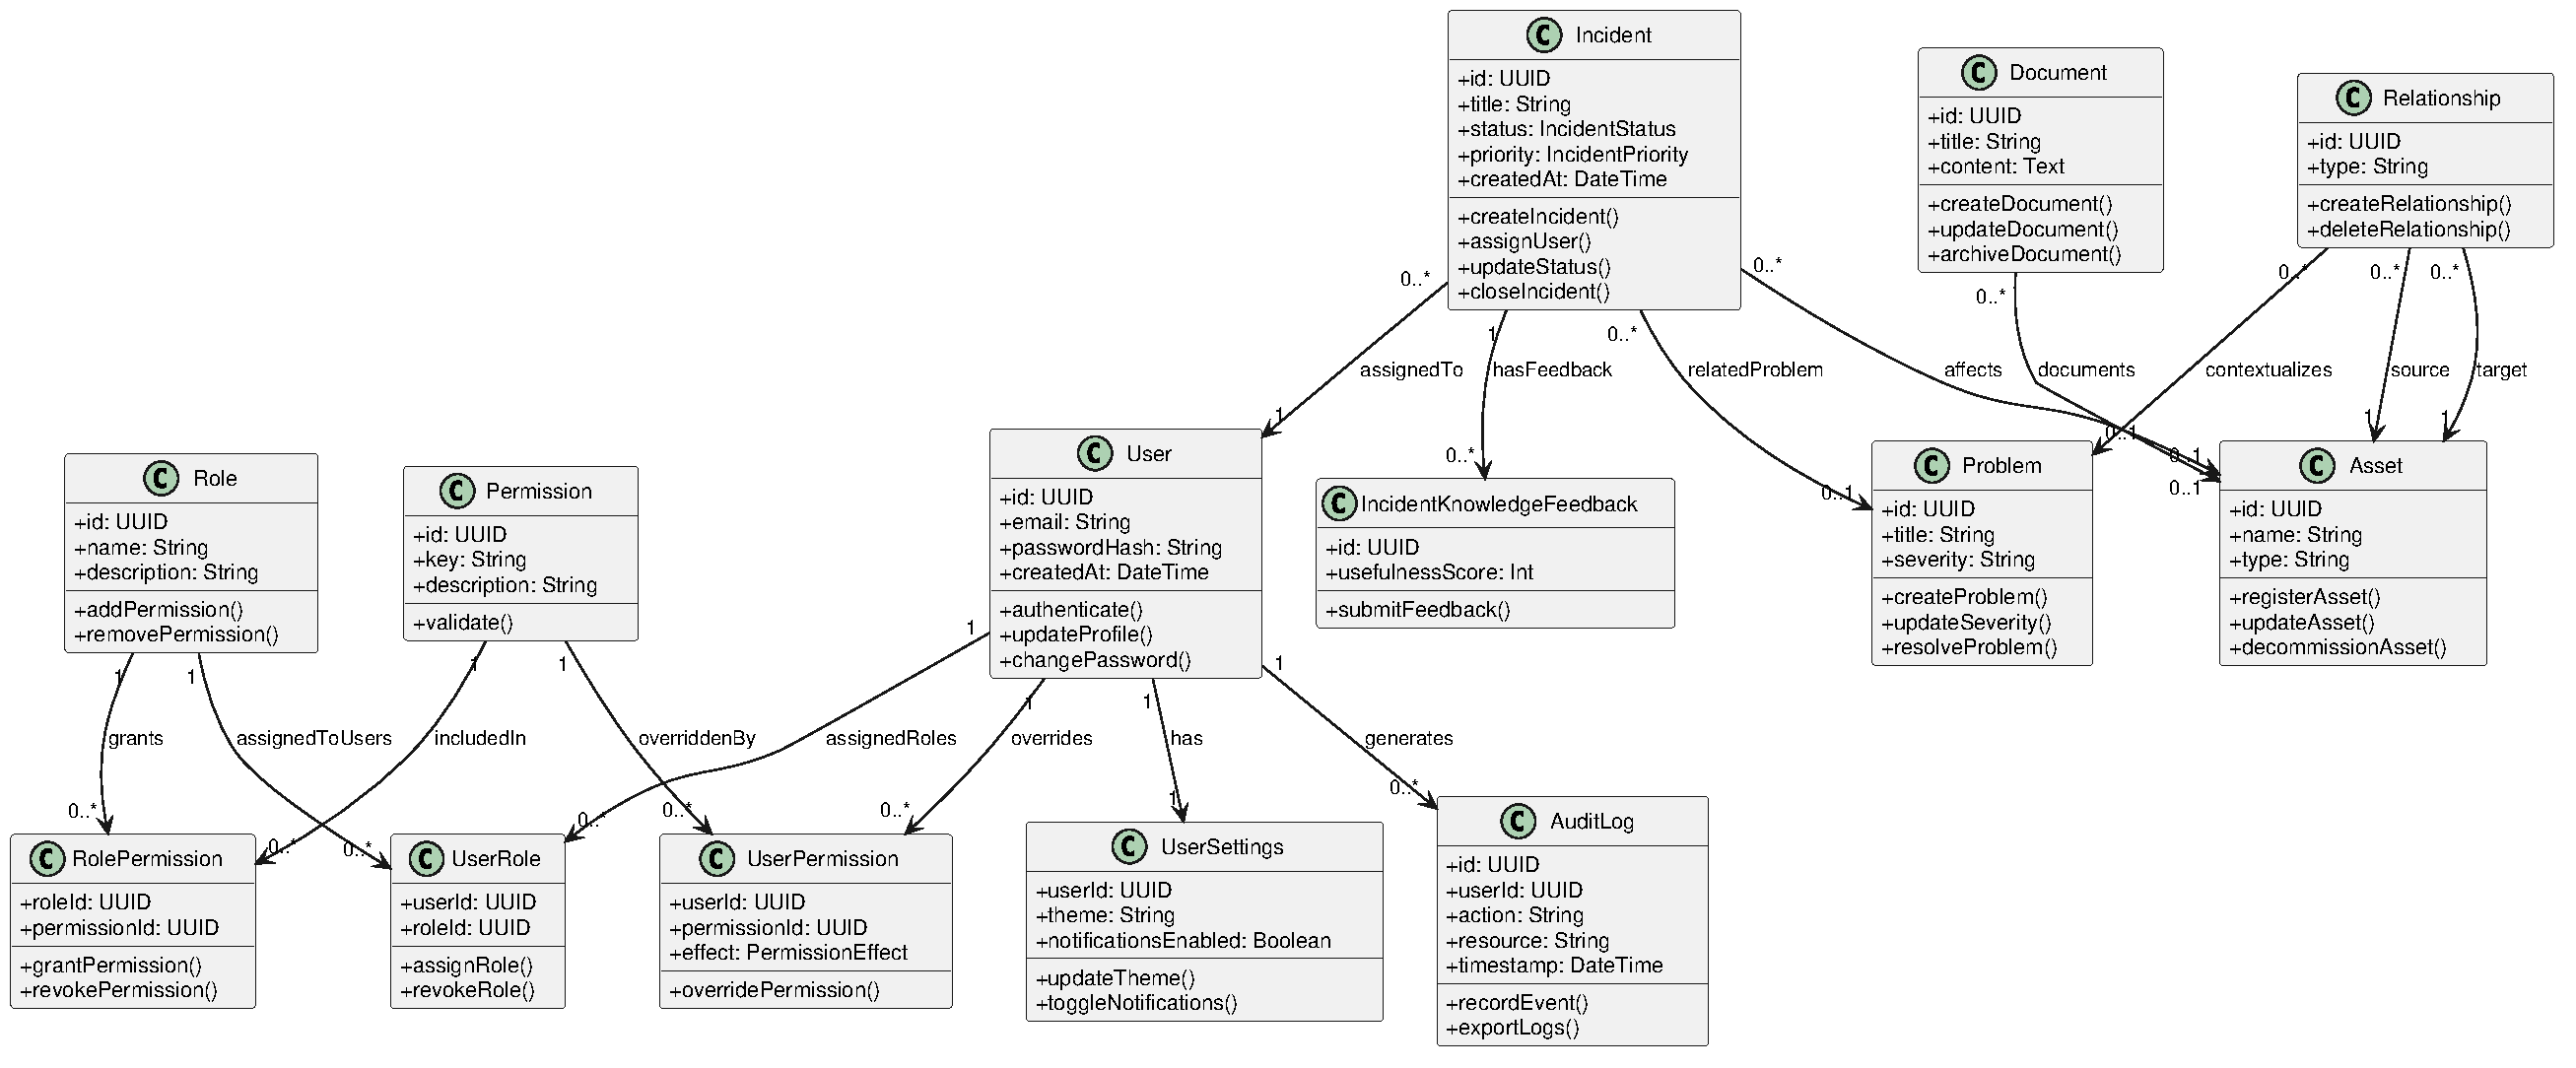
\includegraphics{figures/diagrams/updated_class_diagram.pdf}
    \end{adjustbox}
	\vspace*{\fill}
    \caption{Class diagram of the MapIT domain model}
    \label{fig:class-mapit}
\end{figure}
\end{landscape}


\section{Data Model and Relational Schema}
Once the conceptual model is established, it is translated into a relational schema. This part of the chapter documents the tables, primary keys, foreign keys, cardinalities, and integrity constraints used to preserve consistency in the database. The schema confirms that the persistence layer reflects the behavior described in the use case and class models.

\section{Optional Complementary Diagrams}
Additional diagrams such as activity, component, or deployment diagrams are included when they bring real clarity to the project. In this report, the activity diagram explains a permission-sensitive workflow and complements the other modeling artifacts without adding unnecessary redundancy.

To clarify the permission-governed workflow used in sensitive operations, Figure~\ref{fig:activity-rbac} shows the RBAC activity flow.

\begin{figure}[H]
	\centering
	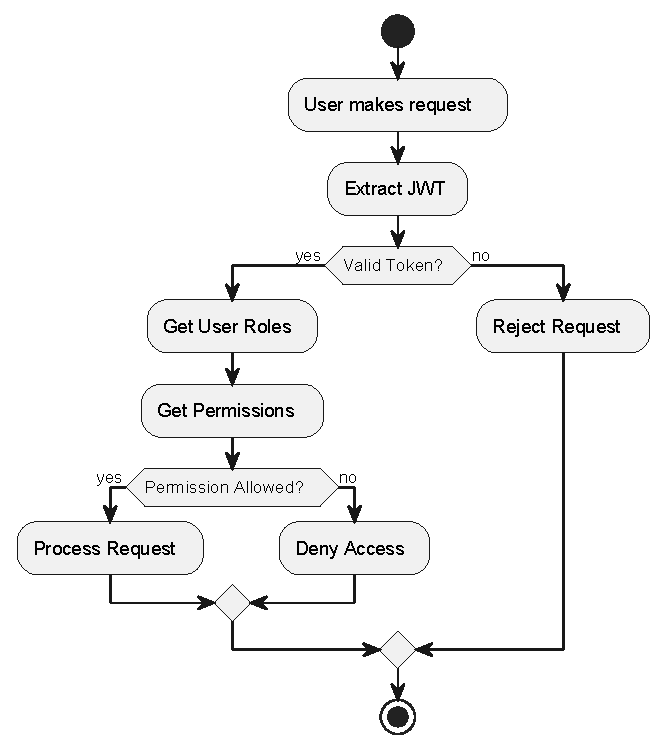
\includegraphics[width=0.95\textwidth]{figures/diagrams/activity_diagram_RBAC.pdf}
	\caption{Activity diagram: RBAC decision flow}
	\label{fig:activity-rbac}
\end{figure}

\section{Chapter Conclusion}
The modeling phase validates the structure of the proposed solution and makes the implementation task more explicit. By separating dynamic behavior, static structure, and data organization, the chapter demonstrates that MapIT has been designed in a disciplined way. The next chapter explains how this design was realized in the actual software stack.

\chapter{Implementation}

\section{Introduction}
This chapter presents the realization of MapIT in the source code. It is intentionally project-specific: the implementation is not described as a generic web application, but as a Next.js 15 and Express.js platform that serves IT infrastructure documentation, incident tracking, asset inventory, relationship mapping, search, reporting, and access control.

\section{Technical Stack and System Architecture}
\subsection{Monorepo structure}
MapIT is organized as a workspace-based monorepo. The main workspace folders are:
\begin{itemize}
	\item \texttt{apps/api}
	\item \texttt{apps/web}
	\item \texttt{apps/mobile}
	\item \texttt{packages/shared}
\end{itemize}
The most important root scripts are:
\begin{itemize}
	\item \texttt{dev:api}, \texttt{dev:web}, \texttt{dev:mobile}
	\item \texttt{typecheck}, \texttt{test:api}, \texttt{smoke:frontend}, \texttt{ci}
\end{itemize}
This structure is important because it separates the operational backend, the browser interface, and the mobile prototype while keeping the project coherent.

\subsection{Web implementation stack}
The web interface uses Next.js 15 with the App Router, React 19, and TypeScript in strict mode. The styling relies on Tailwind CSS 3 and a utility-driven component system, while the state management layer uses Zustand. API calls are made through an Axios client with a 10-second timeout, \texttt{withCredentials} enabled, and a response interceptor that redirects to \texttt{/login} on HTTP 401. The project also uses Lucide icons, React Hook Form, Zod, SWR, TanStack React Query, and Recharts where the UI needs them.

\subsection{Backend implementation stack}
The backend is built on Express 5, Prisma ORM, PostgreSQL, JSON Web Tokens, and ldapjs for Active Directory authentication in production. The server structure is modular: each domain has its own route file under \texttt{apps/api/src/modules/}. There are dedicated modules for authentication, incidents, documents, dashboard summaries, assets, problems, relationships, search, reports, notifications, settings, and administration.

\subsection{Data and persistence layer}
The Prisma schema defines the real MapIT data model. The main entities include:
\begin{itemize}
	\item \texttt{User}, \texttt{Incident}, \texttt{Document}, \texttt{Asset}, \texttt{Problem}, \texttt{Relationship}
	\item \texttt{Role}, \texttt{Permission}, \texttt{UserRole}, \texttt{RolePermission}, \texttt{UserPermission}
	\item \texttt{UserSettings}, \texttt{AuditLog}, and \texttt{IncidentKnowledgeFeedback}
\end{itemize}
This is the persistence layer that makes the platform suitable for technical documentation rather than only for temporary user input.

\section{Authentication and Access Control}
\subsection{Login flow}
The login route accepts a username and password, authenticates against Active Directory through ldapjs when the application is not in development mode, and supports test credentials when \texttt{DEV\_MODE=true}. After successful authentication, the user is upserted in the database, assigned a default role, and issued a JWT valid for one day. The web login page posts to \texttt{/api/auth/login} and then redirects the user to the dashboard.

The login interface is shown in Figure~\ref{fig:ui-login}.

\begin{figure}[H]
	\centering
	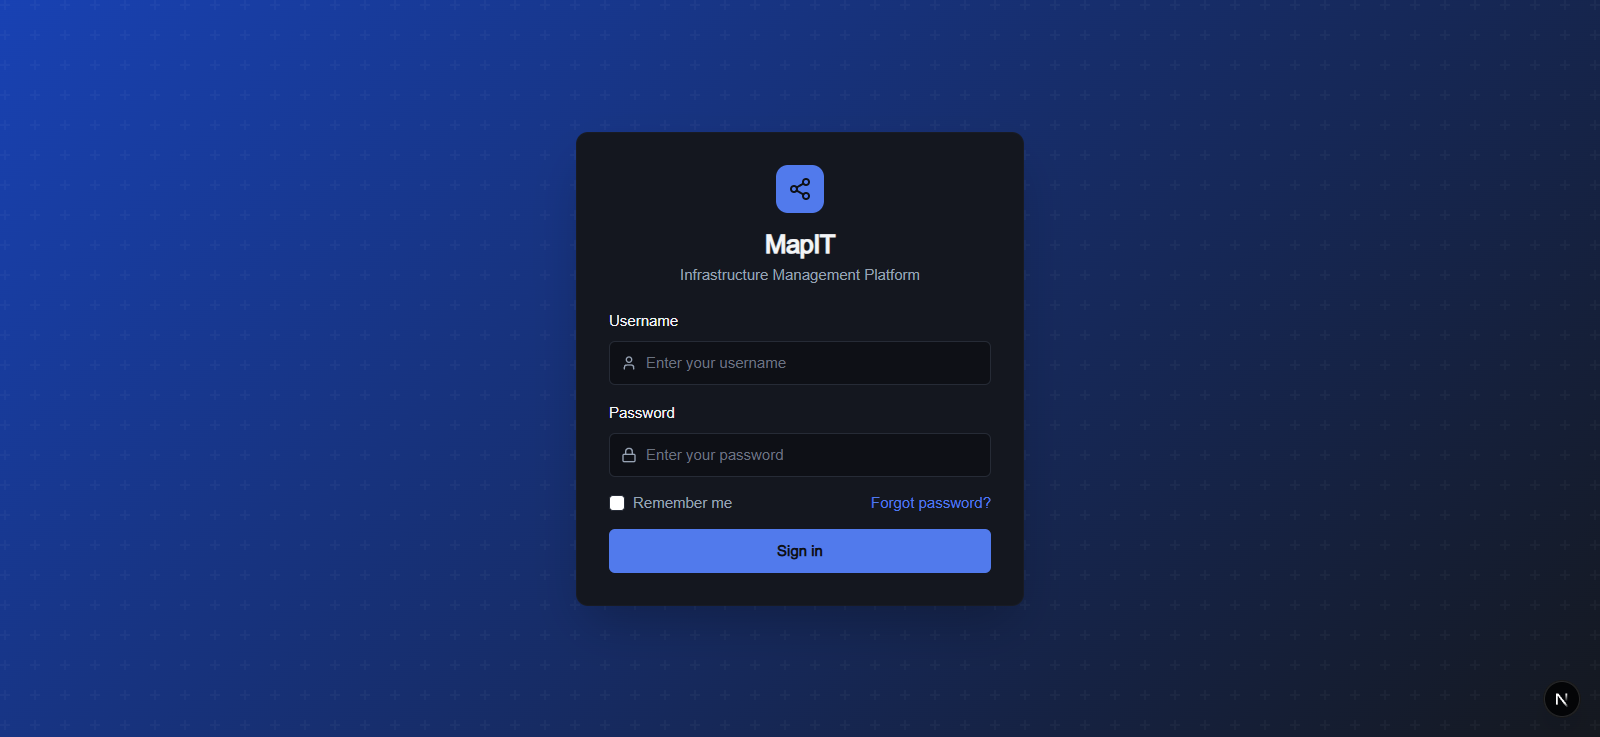
\includegraphics[width=0.9\textwidth]{figures/screenshots/login_page.png}
	\caption{Login page}
	\label{fig:ui-login}
\end{figure}

\subsection{Session and proxy handling}
The frontend does not talk directly to the backend hostname. It sends requests to the Next.js proxy path \texttt{/api/backend/[...path]}, which forwards the browser traffic to the API while keeping the public web application same-origin. The auth store also checks \texttt{/api/auth/session} to determine whether the session is still valid. This is a practical implementation pattern for a secure and deployment-friendly web application.

\subsection{Role-based and permission-based access control}
MapIT goes beyond a simple admin/viewer split. The backend bootstraps permissions and role templates for Admin, Manager, Operator, and Viewer, and it supports user-specific permission overrides. Middleware functions such as \texttt{requireAuth}, \texttt{requireRole}, and \texttt{requirePermission} protect the API. The permission catalog includes fine-grained actions, for example:
\begin{itemize}
	\item \texttt{asset:create}, \texttt{incident:status:update}, \texttt{incident:assign}
	\item \texttt{relationship:create}, \texttt{report:view}, \texttt{settings:update-any}
	\item \texttt{user:manage}, \texttt{permission:manage}
\end{itemize}

Figure~\ref{fig:ui-access-control} illustrates the access-control administration interface used to manage these permission assignments.

\begin{figure}[H]
	\centering
	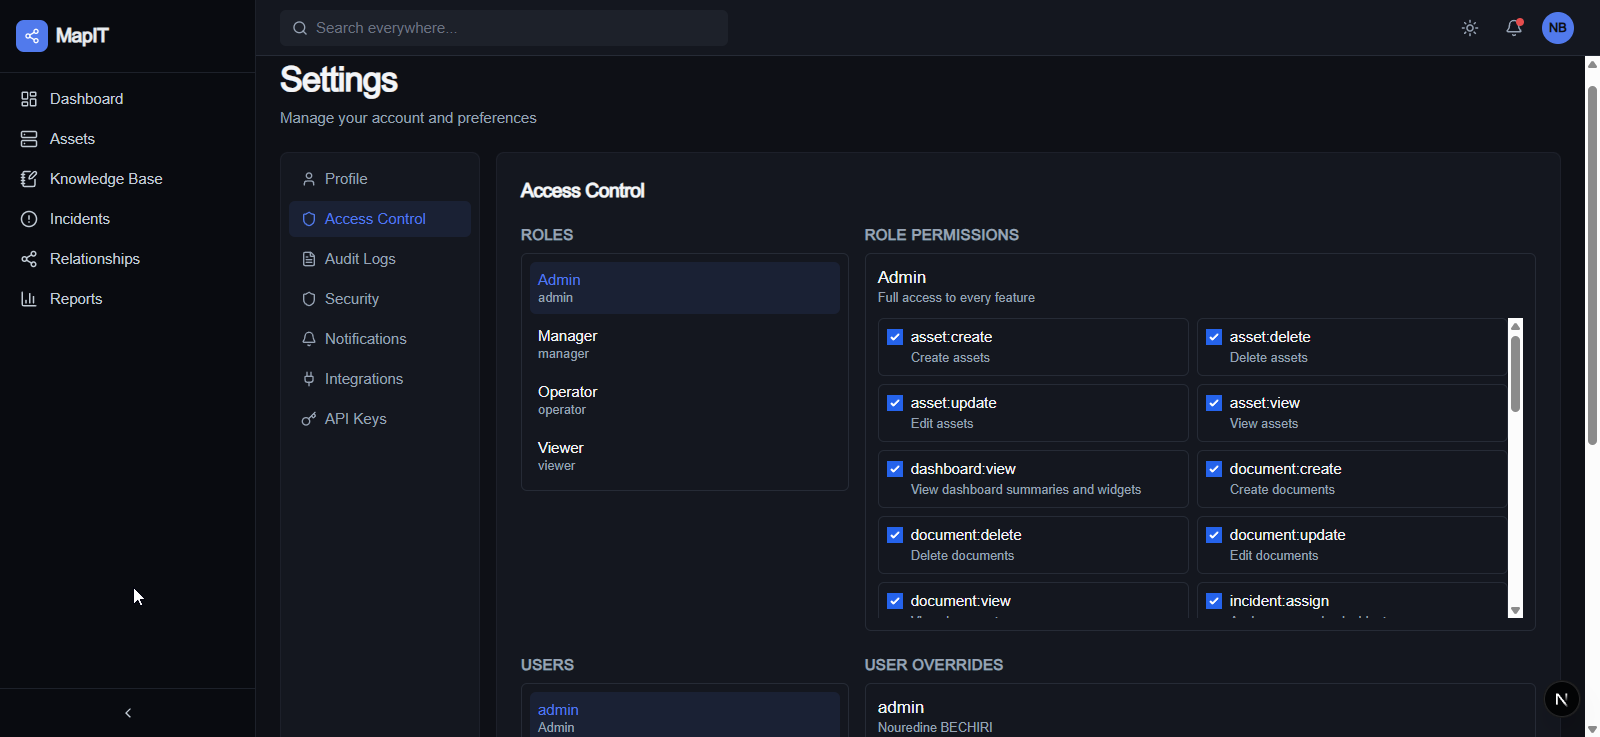
\includegraphics[width=0.95\textwidth]{figures/screenshots/access_control.png}
	\caption{Access control management interface}
	\label{fig:ui-access-control}
\end{figure}

\section{Backend Modules and Business Functions}
\subsection{Incidents}
The incident module is one of the core components of MapIT. It manages incident creation, status transitions, assignment, and knowledge suggestions. The model uses the statuses \texttt{OPEN}, \texttt{IN\_PROGRESS}, \texttt{BLOCKED}, \texttt{RESOLVED}, and \texttt{CLOSED}, together with priorities from \texttt{LOW} to \texttt{CRITICAL}. The detail screen in the web app allows the user to edit the title, description, assigned team, assignee, and status, and it also integrates related knowledge suggestions.

\subsection{Assets and relationships}
The assets module stores infrastructure components such as servers, virtual machines, network devices, storage nodes, and services. The relationship module creates directed connections between assets and returns the graph used by the relationship map page. In the frontend, the map supports dragging nodes, filtering by type, panning, and zooming. This is how MapIT makes infrastructure interdependence visible.

\subsection{Problems and knowledge reuse}
The problems module stores documented problems, affected assets, severity, status, solution text, and resolution dates. This module is the reusable knowledge layer of the application. It is exposed in the Problems page, where users can create, edit, filter, and delete problem entries according to their permissions. The global search module uses these records together with assets, incidents, and documents to produce a unified search result.

\subsection{Search, reports, settings, and audit logs}
The search page performs global search across all knowledge domains. The reports page summarizes assets by type and problems by severity and provides CSV/PDF export. The settings page manages profile data, notifications, theme preferences, access-control administration, and audit-log inspection. The audit trail stores actor, action, resource, and sanitized request metadata so that sensitive operations remain traceable.

The audit trail visualization in Figure~\ref{fig:ui-audit-logs} shows how operational actions remain traceable over time.

\begin{figure}[H]
	\centering
	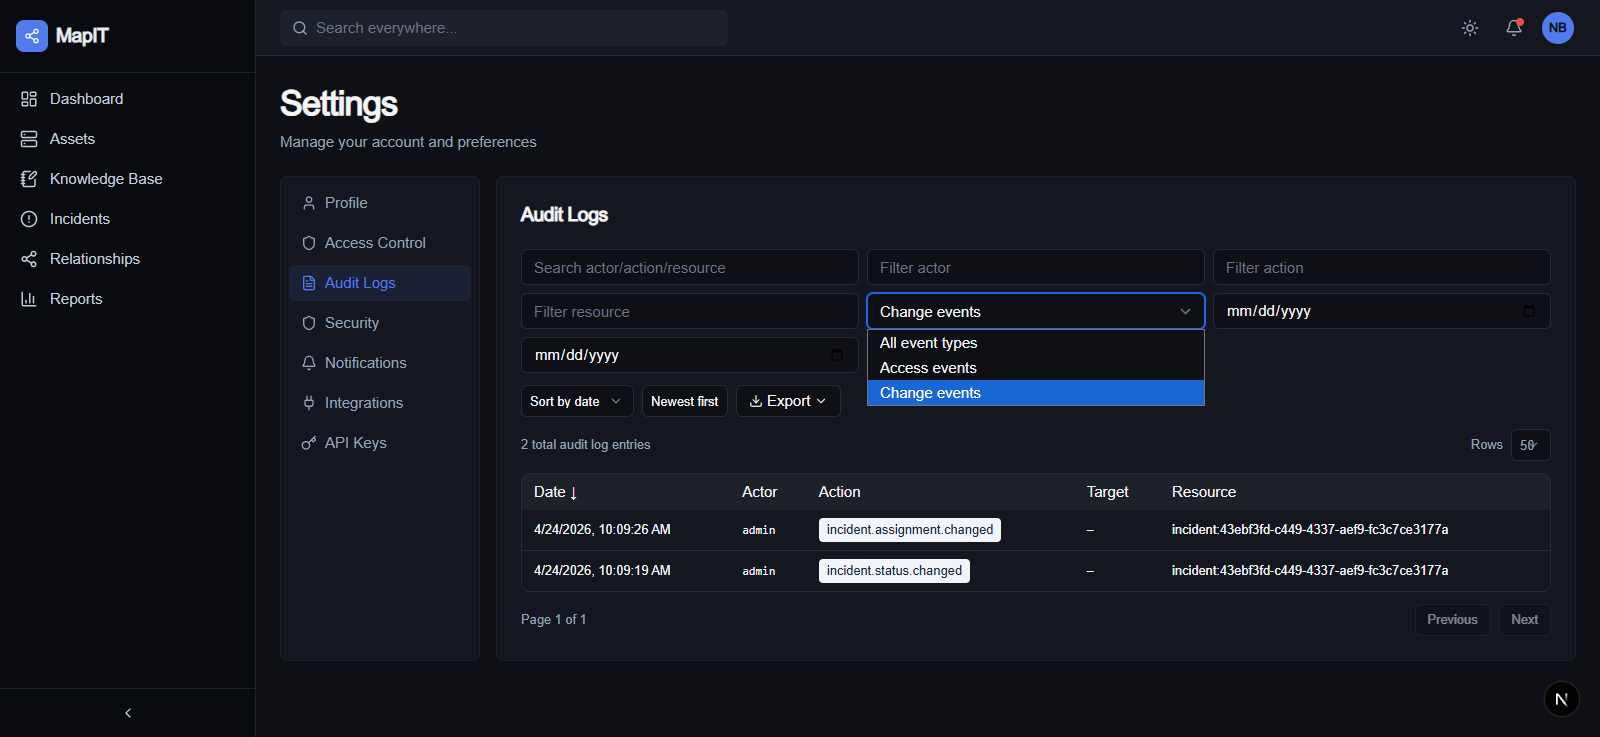
\includegraphics[width=0.95\textwidth]{figures/screenshots/audit_logs.png}
	\caption{Audit logs interface}
	\label{fig:ui-audit-logs}
\end{figure}

\section{Realized User Interfaces}
\subsection{Login and shared layout}
The login page contains a username field, a password field, inline error feedback, and a sign-in button. After authentication, the application redirects to the dashboard. The authenticated pages share a sidebar layout, which is used consistently on the dashboard, incidents, assets, problems, relationships, reports, and settings sections.

\subsection{Dashboard}
The dashboard is not a static welcome page. It loads summary data, assets, and problems in parallel and exposes export actions for CSV and PDF generation. The user can navigate from the dashboard to assets or problems directly, which makes it a control center for the infrastructure team.

\begin{figure}[H]
	\centering
	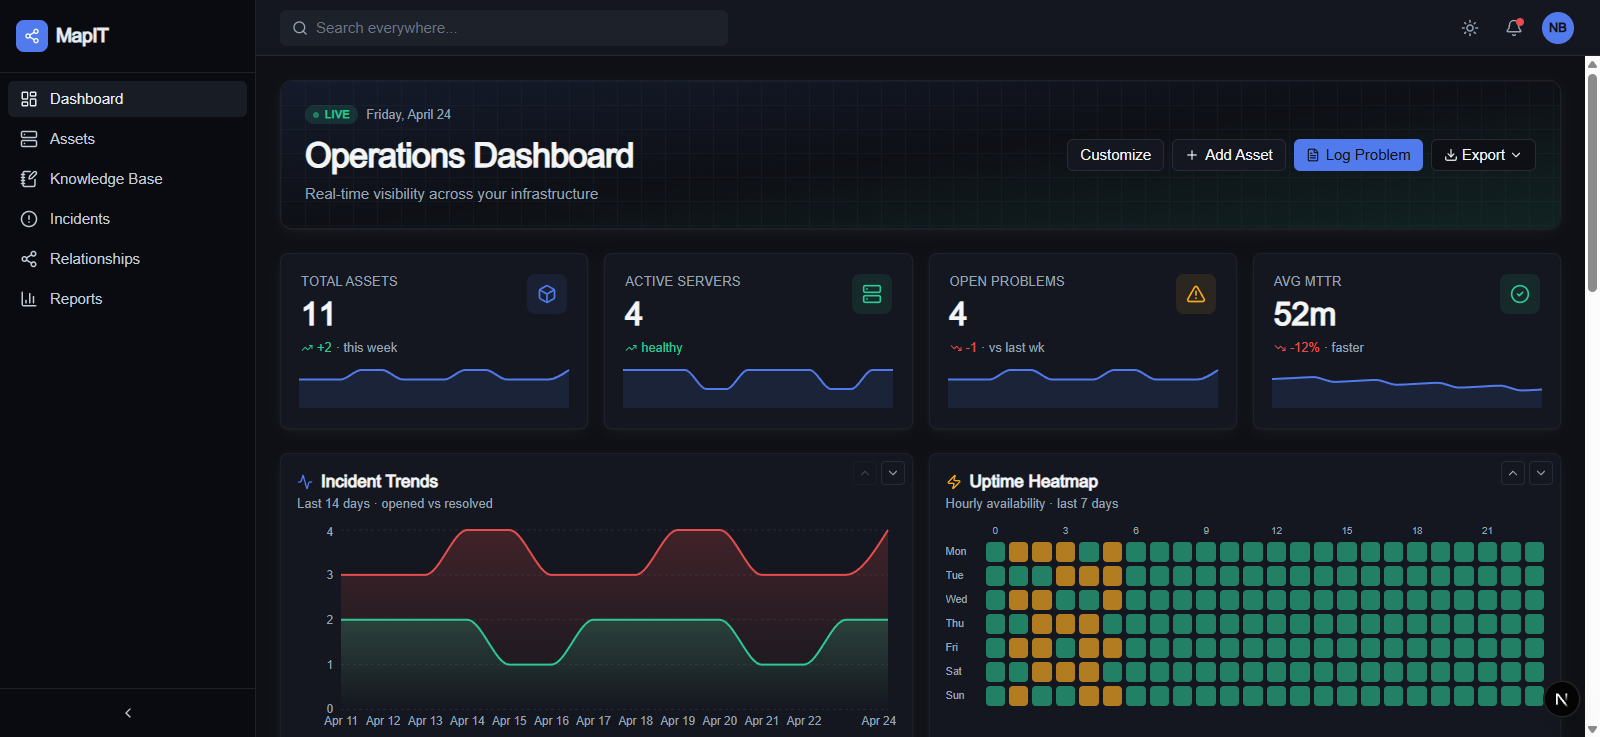
\includegraphics[width=0.95\textwidth]{figures/screenshots/dashboard.png}
	\caption{Dashboard interface}
	\label{fig:ui-dashboard}
\end{figure}

\subsection{Incidents}
The incidents list page supports search by title and description, creation of new incidents, and navigation to incident detail pages. The detail page supports editing, status updates, assignment changes, deletion, and knowledge suggestions. The page also shows status badges and priority badges, which are important for rapid operational reading.

\begin{figure}[H]
	\centering
	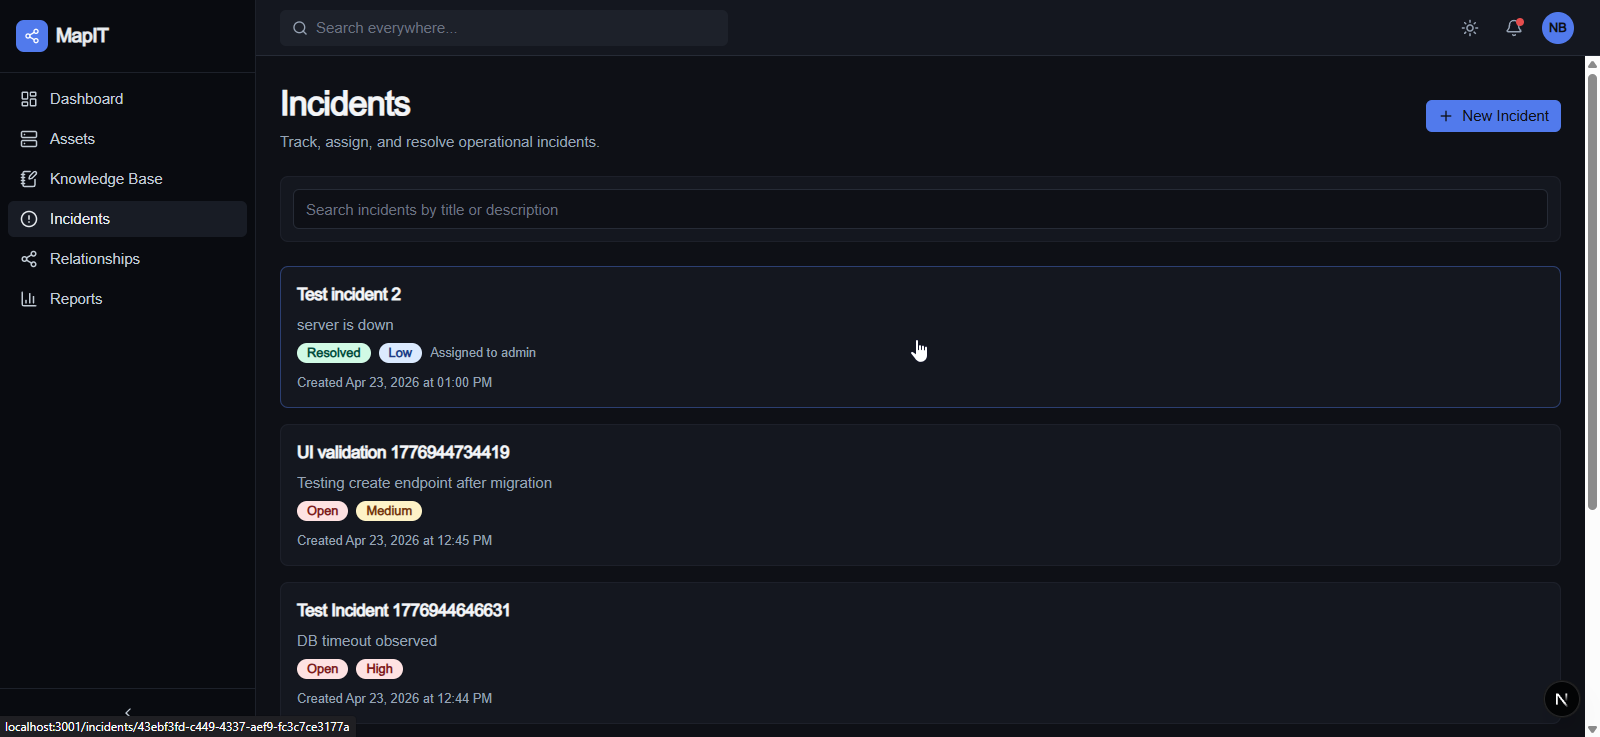
\includegraphics[width=0.95\textwidth]{figures/screenshots/incidents.png}
	\caption{Incidents management interface}
	\label{fig:ui-incidents}
\end{figure}

\subsection{Assets}
The asset inventory page supports filtering, pagination, bulk selection, and an asset creation form that can also create relationships immediately after the asset is saved. The asset detail page shows overview data, related problems, and related assets in separate tabs. The presence of a direct link to the relationship map reinforces the visual nature of the knowledge model.

\begin{figure}[H]
	\centering
	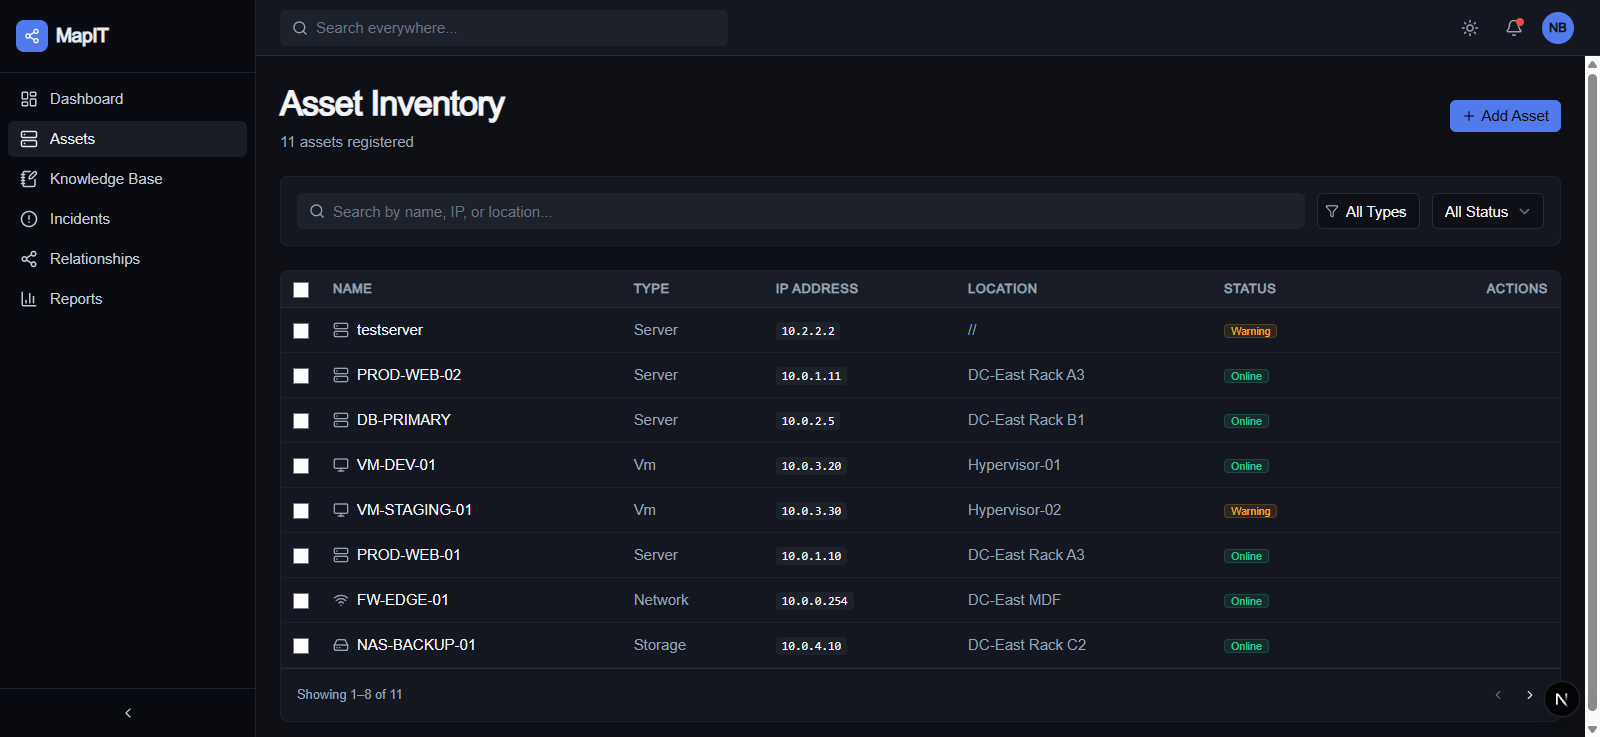
\includegraphics[width=0.95\textwidth]{figures/screenshots/assets.png}
	\caption{Assets inventory interface}
	\label{fig:ui-assets}
\end{figure}

\subsection{Problems, relationships, search, reports, and settings}
The problems page allows the user to manage problem records and associate them with affected assets. The relationships page visualizes the infrastructure graph and supports interactive layout editing. The search page searches across assets, incidents, problems, and documents in one place. The reports page summarizes operational data. The settings page exposes access control, audit logs, security, notifications, integrations, and API-key placeholders.

\begin{figure}[H]
	\centering
	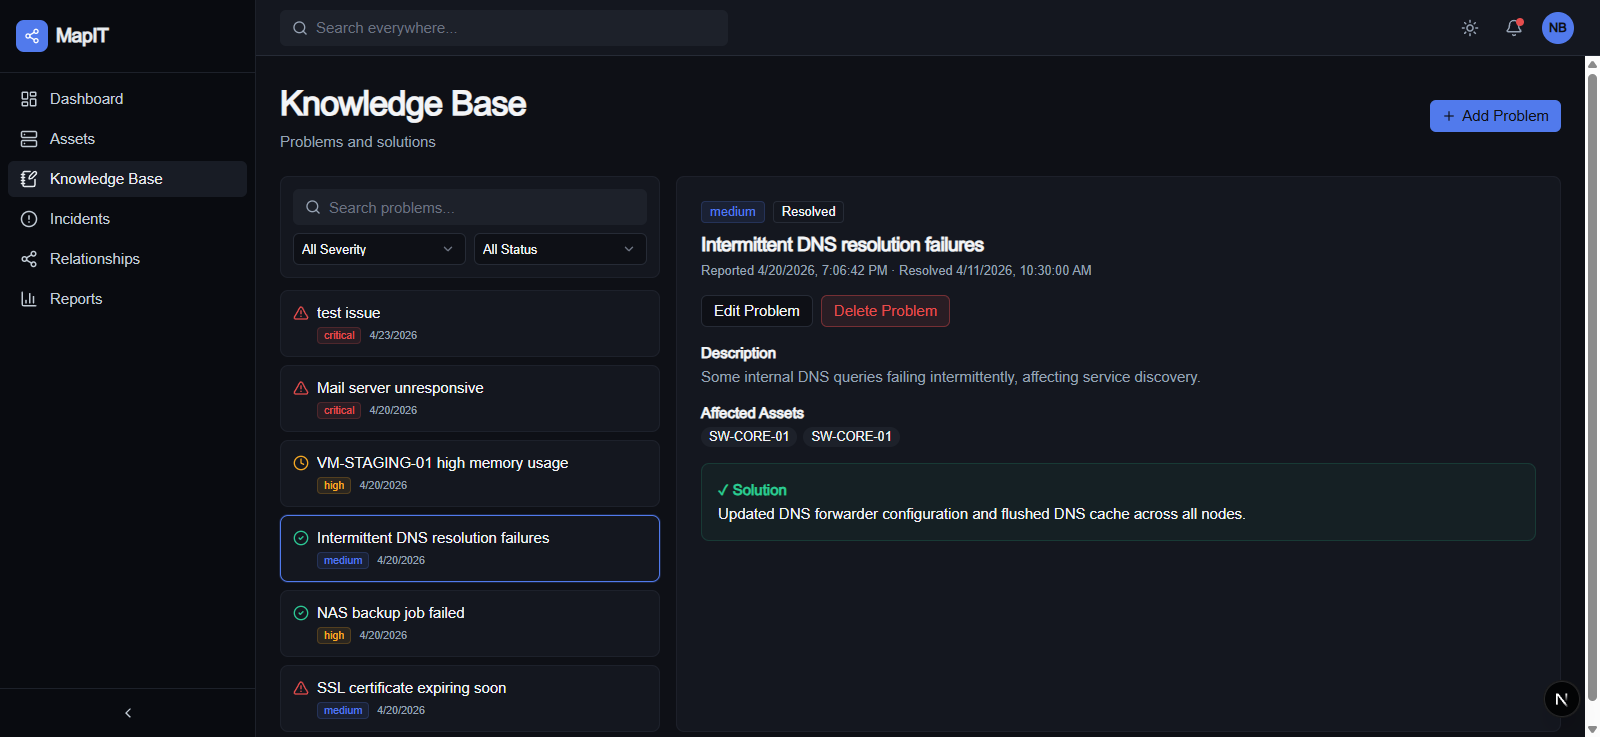
\includegraphics[width=0.95\textwidth]{figures/screenshots/knowledge_base.png}
	\caption{Problem and knowledge base interface}
	\label{fig:ui-knowledge-base}
\end{figure}

\begin{figure}[H]
	\centering
	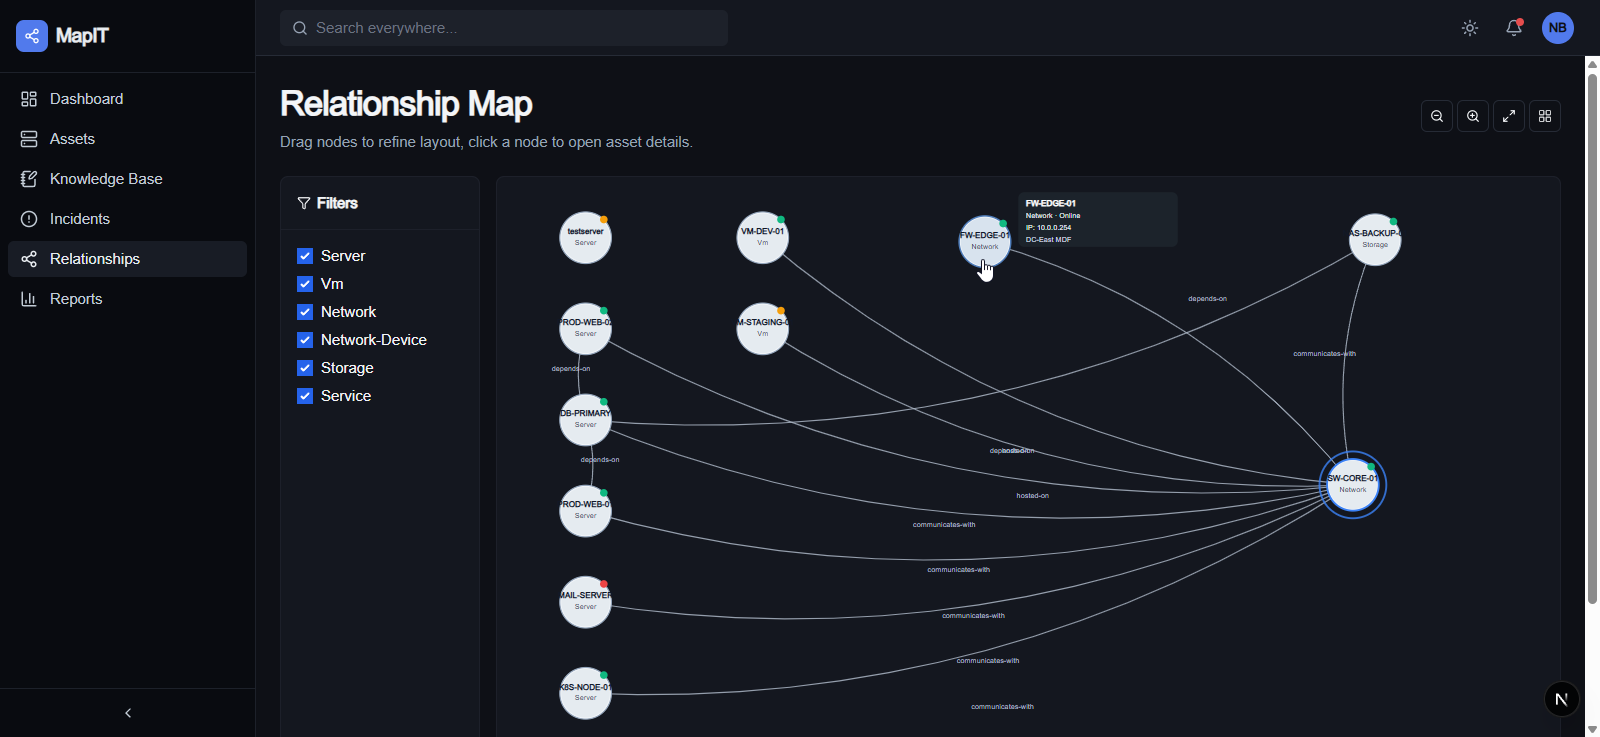
\includegraphics[width=0.95\textwidth]{figures/screenshots/relation_map.png}
	\caption{Relationship map interface}
	\label{fig:ui-relationship-map}
\end{figure}

\begin{figure}[H]
	\centering
	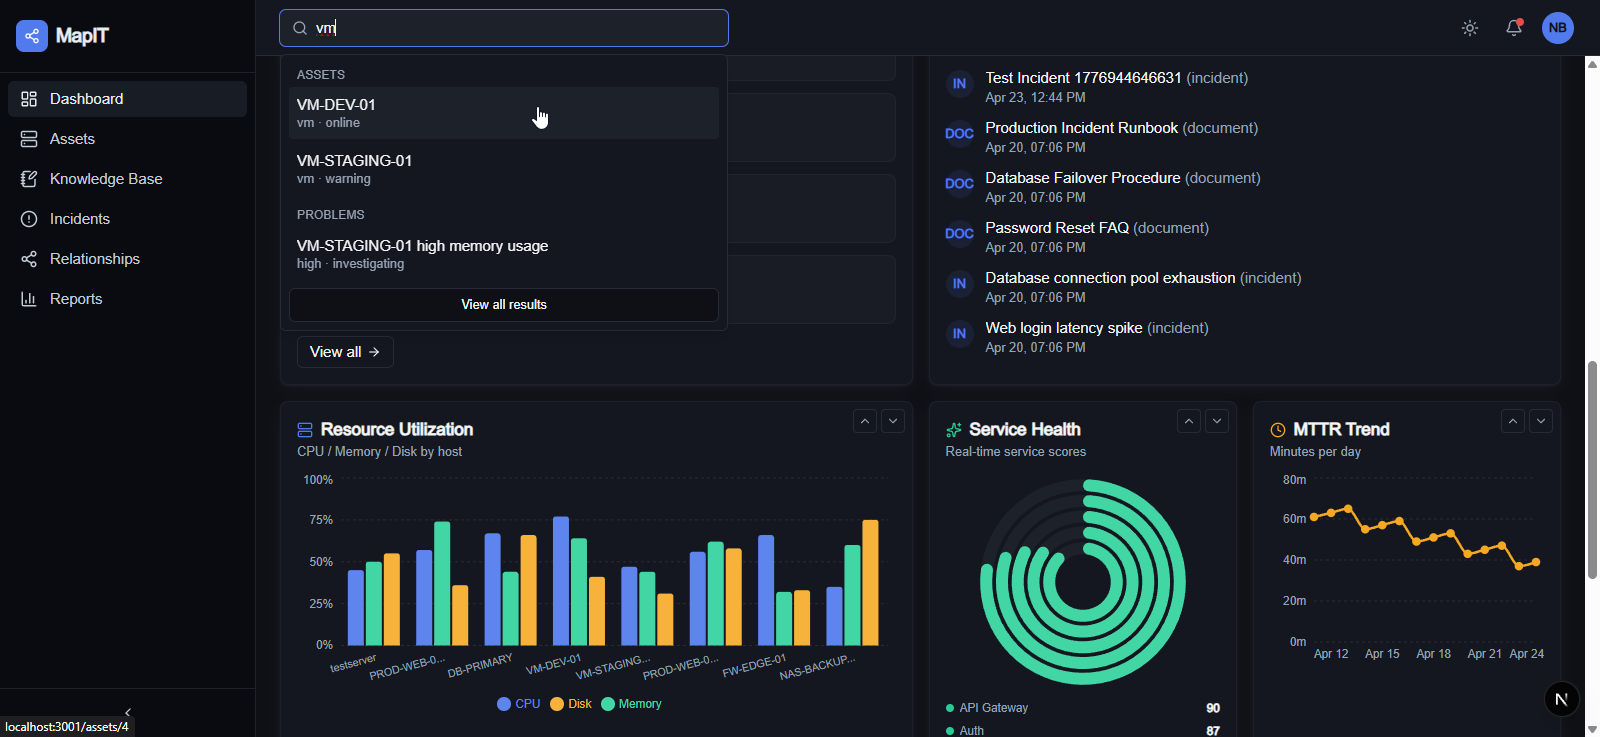
\includegraphics[width=0.95\textwidth]{figures/screenshots/search.png}
	\caption{Global search interface}
	\label{fig:ui-search}
\end{figure}

\begin{figure}[H]
	\centering
	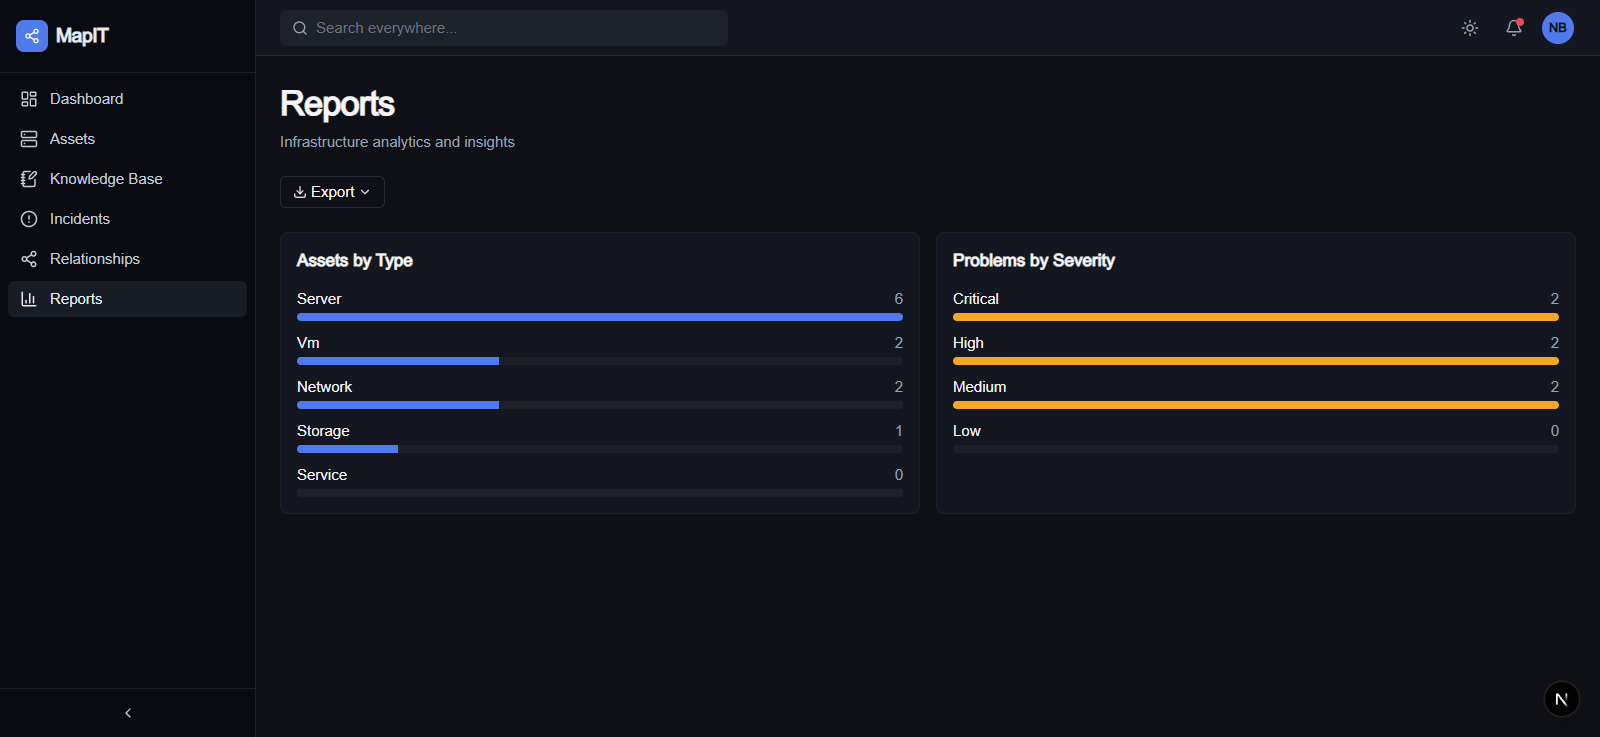
\includegraphics[width=0.95\textwidth]{figures/screenshots/reports.png}
	\caption{Reports interface}
	\label{fig:ui-reports}
\end{figure}

\section{Deployment and Execution Notes}
\subsection{Local execution}
The local development workflow is explicit: \texttt{npm run dev:api} starts the API on port 3000, \texttt{npm run dev:web} starts the web app on port 3001, and the root scripts support linting, type checking, integration testing, and smoke testing. This is consistent with the way the application is meant to be maintained during development.

\subsection{Environment and configuration}
The backend requires \texttt{DATABASE\_URL}, \texttt{JWT\_SECRET}, \texttt{AD\_URL}, \texttt{AD\_DOMAIN}, \texttt{CORS\_ORIGIN}, \texttt{ADMIN\_USERNAMES}, and \texttt{DEV\_MODE}. The web layer uses the proxy base \texttt{/api/backend} and the session route \texttt{/api/auth/session}. These configuration points are evidence that the project is already organized for a real deployment scenario.

\subsection{Production orientation}
The README describes deployment readiness on Vercel for the web application, Docker for the API, and Expo builds for the mobile prototype. The implementation chapter should therefore present MapIT as a deployable system rather than as a code-only exercise.

\section{Validation and Testing}
\subsection{Backend checks}
The backend uses integration tests under the Node test runner, and Prisma generation is part of the backend lifecycle. The audit logger, permission middleware, and authentication route can all be exercised through API requests, which is a strong basis for validation.

\subsection{Frontend checks}
The web app supports TypeScript type checking, linting, Playwright end-to-end testing, and smoke-style validation. These checks are useful because MapIT’s value depends not only on the backend data model but also on whether users can navigate the real pages effectively.

\section{Chapter Conclusion}
The implementation of MapIT is specific, structured, and aligned with the project’s academic objective. It combines a secure backend, a modern web frontend, a normalized data model, graph-based relationship mapping, global search, reporting, and access control. The next and final chapter can now synthesize the contribution of the project and outline future improvements.


\chapter*{General Conclusion}
\addcontentsline{toc}{chapter}{General Conclusion}
MapIT was designed to address a practical need that appears frequently in IT environments: the difficulty of keeping infrastructure documentation and incident knowledge in one reliable place. By combining a structured data model, role-aware access, and a clear web interface, the project demonstrates how a focused application can improve knowledge reuse and support operational continuity. The work also shows how theoretical concepts such as incident management, knowledge governance, and modeling translate into a coherent software solution.

From a practical point of view, the application establishes a foundation that can be extended with richer search, asset relationships, analytics, workflow automation, and stronger reporting features. These improvements would strengthen the product beyond the academic prototype and move it closer to a complete operational knowledge platform.


% -----------------------------------------------------------------------------
% Bibliography
% -----------------------------------------------------------------------------
\bibliographystyle{plain}
\bibliography{references}

\end{document}
